\documentclass[lang=cn,10pt]{elegantbook}

%%%%%%%%%%%%%%%%%%%%%%%%%%%%%%%%%%%%%%%%%%%%%%%%%%%%%%%%%%%%%%%%%%%%%%%%%%%%%%
%% 包设置
%%%%%%%%%%%%%%%%%%%%%%%%%%%%%%%%%%%%%%%%%%%%%%%%%%%%%%%%%%%%%%%%%%%%%%%%%%%%%%
\usepackage[ruled,noline]{algorithm2e} % 算法包
%\setlength{\lineskip}{2em} %设置行间距
\setlength{\parskip}{0.7em} %设置段落间距

% 本文档命令
\usepackage{array}
\newcommand{\ccr}[1]{\makecell{{\color{#1}\rule{1cm}{1cm}}}}

%%%%%%%%%%%%%%%%%%%%%%%%%%%%%%%%%%%%%%%%%%%%%%%%%%%%%%%%%%%%%%%%%%%%%%%%%%%%%%
%% 封面设置
%%%%%%%%%%%%%%%%%%%%%%%%%%%%%%%%%%%%%%%%%%%%%%%%%%%%%%%%%%%%%%%%%%%%%%%%%%%%%%
\title{Python 3.10 代码分析}
\author{kenshinl}
\date{Last Update: \today}
\version{0.1}
\bioinfo{封面图片作者}{Elina Bernpaintner}
\extrainfo{人生代代无穷已,江月年年望相似。}
\setcounter{tocdepth}{3}
\cover{cover.jpg}
% 修改标题页的橙色带
\definecolor{customcolor}{RGB}{255, 255, 255}
\colorlet{coverlinecolor}{customcolor}

\begin{document}
\maketitle
\frontmatter
\tableofcontents
\mainmatter


% TODO LIST
% 添加一节介绍 GIL 的实现

%%%%%%%%
% draw.io导出图像标准
% png 400ppi 边框宽度为 5 非透明


\chapter{环境准备}

本书对 Python 3.10.4 版本的代码实现进行探究。使用的 Python 实现为 CPython。

\section{Python 编译}

为了了解 Python 的细节,探究和验证代码的实现是否符合自己的预期,我们需要亲自动手修改源码,添加测试代码。
为了完成这个目的,需要学会自己动手编译 Python 源码。所以在本节,将介绍如何编译 Python 代码。

\subsection{在 Linux/MacOS 平台上编译 Python}

编译步骤如下:

第一步是下载 Python 代码并切换到 Python 3.10.4 版本。

\begin{lstlisting}[language=bash, numbers=left, numbersep=1em, numberstyle=\footnotesize , breaklines=true]
# 从 github 克隆代码
$ git clone https://github.com/python/cpython.git
# 切换到 v3.10.4
$ git checkout v3.10.4
# 查看是否切换成功,如下所示就表示成功切换到了 v3.10.4 的代码
$ git branch
* (HEAD detached at v3.10.4)
  main
\end{lstlisting}

第二步就是进行代码的编译

\begin{lstlisting}[language=bash, numbers=left, numbersep=1em, numberstyle=\footnotesize , breaklines=true]
# 进入 cpython 代码目录
cd cpython
# 根据当前系统环境,生成带 debug 信息的 Makefile 
$ ./configure --with-pydebug
# 编译代码
$ make -j8
\end{lstlisting}

在编译完成之后,可以在当前目录看到一个叫做 python.exe 的文件(在 Linux 系统下,编译出来的可执行文件名是 python),
这个文件就是我们正常使用的 Python 程序了。

接下来,你可以使用这个程序进行一些 Python 代码的测试。

\begin{lstlisting}[language=bash, numbers=left, numbersep=1em, numberstyle=\footnotesize , breaklines=true]
$ ./python.exe
Python 3.10.4 (tags/v3.10.4:9d38120e33, May 15 2022, 02:03:06) [Clang 13.0.0 (clang-1300.0.29.30)] on darwin
Type "help", "copyright", "credits" or "license" for more information.
>>> print("test print")
test print
>>> print(2**3)
8
\end{lstlisting}


\begin{definition}[编译过程中的警告] \label{def:int}
在编译的过程中,如果提示 ssh、 \_lzma 等少数几个模块没有 build 成功的话也没有关系,不会影响后面的讲解。只要 python.exe 文件
成功编译出来即可。也可以通过在终端最后几行的输出中查找是否有 "Python build finished successfully!" 字样来判断是否编译成功。
\end{definition}


\section{文档编译}

在学习 cpython 源代码的过程中,如果能阅读相关模块的设计文档可以起到事半功倍的作用,所幸 cpython 考虑到了这一点,为我们准备好了丰富的
文档来辅助学习。cpython 的文档都放置在 cpython/Doc 路径下,以 rst 文件的纯文本格式保存。如果不想直接看 rst 文件,可以将文档编译为其他
的格式。下面就是 cpython 文档支持的转换格式。

\begin{lstlisting}[language=bash, numbers=left, numbersep=1em, numberstyle=\footnotesize , breaklines=true]
$ make
Please use `make <target>' where <target> is one of
  clean      to remove build files
  venv       to create a venv with necessary tools
  html       to make standalone HTML files
  htmlview   to open the index page built by the html target in your browser
  htmlhelp   to make HTML files and a HTML help project
  latex      to make LaTeX files, you can set PAPER=a4 or PAPER=letter
  text       to make plain text files
  texinfo    to make Texinfo file
  epub       to make EPUB files
  changes    to make an overview over all changed/added/deprecated items
  linkcheck  to check all external links for integrity
  coverage   to check documentation coverage for library and C API
  doctest    to run doctests in the documentation
  pydoc-topics  to regenerate the pydoc topics file
  dist       to create a "dist" directory with archived docs for download
  suspicious to check for suspicious markup in output text
  check      to run a check for frequent markup errors
  serve      to serve the documentation on the localhost (8000)
\end{lstlisting}

对通常的开发者来说,编译为 HTML 就足够了,可以在阅读源代码的同时使用浏览器查看对应的文档。编译为 HTML 的方式也很简单,只需要
在 cpython/Doc 目录下执行 make htmlview 即可,编译出的 HTML 格式文档保存在 cpython/Doc/build/html 目录下,使用浏览器打开这个
目录下的 index.html 文件即可看到文档内容。

\begin{definition}[rst 文件] \label{def:int}
rst 是 reStructuredText 的缩写,reStructuredText 是一种易于阅读,所见即所得的纯文本标记语法和解析器系统。reStructuredText 的主要目标
是定义和实现用于 Python 文档字符串和其他文档域的标记语法,该语法可读且简单,但足够强大,可以轻松使用。通俗来说,reStructuredText
 是一种和 markdowm 类似的标记语法,rst 文件是一种和 markdown 文档类似的纯文本文档。
\end{definition}

\section{dis 工具}

本节介绍下 dis 工具的使用。

\section{静态值工具}

本节介绍开发一个分析静态数据的工具。

\section{参考资料}

\begin{itemize}
\item \href{https://peps.python.org/pep-0006/}{PEP 6 – Bug Fix Releases}
\item \href{https://docutils.sourceforge.io/rst.html}{reStructuredText-Markup Syntax and Parser Component of Docutils}
\end{itemize}
 % 环境准备
%\chapter{一些概念和问题}

\section*{First集和Follow集的作用}


\subsection*{算法实现}

\begin{algorithm}[H]
    \renewcommand{\thealgocf}{}
    \caption{\texttt{求nullable、FIRST 集和 FOLLOW 集}}
%    \KwIn{None}
%    \KwOut{None}
将所有的 FIRST 和 FOLLOW 集合初始化为空,将所有的 nullable 初始化为 false \\
\For {每一个终结符 $Z$} {
	$FIRST[Z] \leftarrow \{Z\}$
}

\Repeat {$FIRST$ 、$FOLLOW$ 和 $nullable$ 在此轮迭代中没有改变} {
\For {每个产生式 $X \rightarrow Y_{1}Y_{2} \cdots Y_{k}$} {
	\For {每个 $i$ 从 $1$ 到 $k$,每个 $j$ 从$i+1$到$k$} {
		\If {所有 $Y_{i}$都是可为空的}{
			$nullable[X] \leftarrow true$ \\
		}
		\If {$Y_{1} \cdots Y_{i-1}$都是可为空的}{
			$FIRST[X] \leftarrow FIRST[X] \cup FIRST[Y_{i}]$ \\
		}
		\If {$Y_{i+1} \cdots Y_{k}$ 都是可为空的}{
			$FOLLOW[Y_{i}] \leftarrow FOLLOW[Y_{i}] \cup FOLLW[X]$ \\
		}
		\If {$Y_{i+1} \cdots Y_{j-1}$都是可为空的}{
			$FOLLOW[Y_{i}] \leftarrow FOLLOW[Y_{i}] \cup FIRST[Y_{j}]$ \\
		}
	}
}
}

\end{algorithm}



\section*{词法分析和语法分析的关联体现在什么地方}


\section*{左递归带来的问题是什么}

要搞清楚这个问题,首先需要知道什么是左递归。左递归的定义如下:

对于上下文无关文法的一个规则来说,如果其右侧第一个符号与左侧符号相同或者能够推导出左侧符号,
那么称该规则为左递归的。前一种情况称为直接左递归,后一种情况成为间接左递归。



以一个经典的包含左递归的表达式语法为例。

\begin{lstlisting}[caption={经典表达式文法}]
Goal   -> Expr
Expr   -> Expr + Term
Expr   |  Expr - Term
       |  Term
Term   -> Term * Factor
Term   |  Term / Factor
       |  Factor
Factor -> ( Expr )
       |  num
       | name
\end{lstlisting}

左递归是自顶向下语法分析中需要专门处理的一个问题。自定向下语法语法分析是指从语法分析树的根开始,
系统地向下拓展树,直至树的叶结点与词法分析器返回地已归类单词相匹配。在过程的每一点上,都需要考虑
一个部分完成的语法分析树。过程在树的下边缘选择一个非终结符,选定某个适用于该非终结符的产生式,用
与产生式右侧相对应的子树来拓展该结点。终结符是无法拓展的。这个过程会一直持续下去,直到语法分析树
的下边缘只包含终结符,且输入流已经耗尽。

从上面的描述中可以看出,自顶向下语法分析的关键就是选择一个合适的非终结符进行拓展。以句子
a+b*c 为例,了解左递归对自顶向下语法分析带来的问题。

\begin{lstlisting}[caption={自顶向下语法分析 a+b*c}]
规则0  Expr
规则1  Expr + Term
规则1  Expr + Term + Term
规则1  Expr + Term + Term + Term
...
\end{lstlisting}

在第二行开始,语法分析器知道非终结符 Expr 和输入单词 a,它选择规则1进行匹配,在第三行,语法分析器
还是面临非终结符 Expr 和输入单词 a,他继续选择规则1进行匹配,导致了无限循环。这也就是左递归给自顶向下
语法分析带来的问题。在这个例子中,语法分析器向前多看一个单词在这里可以解决问题,但是如果语法足够复杂,
左递归仍然会导致这个问题。所以,需要有一个算法来消除左递归。对于直接左递归,可以采用如下的方式。

\begin{lstlisting}[caption={消除直接左递归}]
Fee -> Fee @($\alpha$)@
    |  @($\beta$)@
    
转换为如下产生式

Fee  -> @($\beta$)@ Fee'
Fee' -> @($\alpha$)@ Fee'
     |  @($\epsilon$)@
\end{lstlisting}

对于间接左递归的消除算法就不在这里描述了。

\section*{什么是递归下降分析器}
 % 字节码介绍
\chapter{一些概念和问题}

\section*{First集和Follow集的作用}


\subsection*{算法实现}

\begin{algorithm}[H]
    \renewcommand{\thealgocf}{}
    \caption{\texttt{求nullable、FIRST 集和 FOLLOW 集}}
%    \KwIn{None}
%    \KwOut{None}
将所有的 FIRST 和 FOLLOW 集合初始化为空,将所有的 nullable 初始化为 false \\
\For {每一个终结符 $Z$} {
	$FIRST[Z] \leftarrow \{Z\}$
}

\Repeat {$FIRST$ 、$FOLLOW$ 和 $nullable$ 在此轮迭代中没有改变} {
\For {每个产生式 $X \rightarrow Y_{1}Y_{2} \cdots Y_{k}$} {
	\For {每个 $i$ 从 $1$ 到 $k$,每个 $j$ 从$i+1$到$k$} {
		\If {所有 $Y_{i}$都是可为空的}{
			$nullable[X] \leftarrow true$ \\
		}
		\If {$Y_{1} \cdots Y_{i-1}$都是可为空的}{
			$FIRST[X] \leftarrow FIRST[X] \cup FIRST[Y_{i}]$ \\
		}
		\If {$Y_{i+1} \cdots Y_{k}$ 都是可为空的}{
			$FOLLOW[Y_{i}] \leftarrow FOLLOW[Y_{i}] \cup FOLLW[X]$ \\
		}
		\If {$Y_{i+1} \cdots Y_{j-1}$都是可为空的}{
			$FOLLOW[Y_{i}] \leftarrow FOLLOW[Y_{i}] \cup FIRST[Y_{j}]$ \\
		}
	}
}
}

\end{algorithm}



\section*{词法分析和语法分析的关联体现在什么地方}


\section*{左递归带来的问题是什么}

要搞清楚这个问题,首先需要知道什么是左递归。左递归的定义如下:

对于上下文无关文法的一个规则来说,如果其右侧第一个符号与左侧符号相同或者能够推导出左侧符号,
那么称该规则为左递归的。前一种情况称为直接左递归,后一种情况成为间接左递归。



以一个经典的包含左递归的表达式语法为例。

\begin{lstlisting}[caption={经典表达式文法}]
Goal   -> Expr
Expr   -> Expr + Term
Expr   |  Expr - Term
       |  Term
Term   -> Term * Factor
Term   |  Term / Factor
       |  Factor
Factor -> ( Expr )
       |  num
       | name
\end{lstlisting}

左递归是自顶向下语法分析中需要专门处理的一个问题。自定向下语法语法分析是指从语法分析树的根开始,
系统地向下拓展树,直至树的叶结点与词法分析器返回地已归类单词相匹配。在过程的每一点上,都需要考虑
一个部分完成的语法分析树。过程在树的下边缘选择一个非终结符,选定某个适用于该非终结符的产生式,用
与产生式右侧相对应的子树来拓展该结点。终结符是无法拓展的。这个过程会一直持续下去,直到语法分析树
的下边缘只包含终结符,且输入流已经耗尽。

从上面的描述中可以看出,自顶向下语法分析的关键就是选择一个合适的非终结符进行拓展。以句子
a+b*c 为例,了解左递归对自顶向下语法分析带来的问题。

\begin{lstlisting}[caption={自顶向下语法分析 a+b*c}]
规则0  Expr
规则1  Expr + Term
规则1  Expr + Term + Term
规则1  Expr + Term + Term + Term
...
\end{lstlisting}

在第二行开始,语法分析器知道非终结符 Expr 和输入单词 a,它选择规则1进行匹配,在第三行,语法分析器
还是面临非终结符 Expr 和输入单词 a,他继续选择规则1进行匹配,导致了无限循环。这也就是左递归给自顶向下
语法分析带来的问题。在这个例子中,语法分析器向前多看一个单词在这里可以解决问题,但是如果语法足够复杂,
左递归仍然会导致这个问题。所以,需要有一个算法来消除左递归。对于直接左递归,可以采用如下的方式。

\begin{lstlisting}[caption={消除直接左递归}]
Fee -> Fee @($\alpha$)@
    |  @($\beta$)@
    
转换为如下产生式

Fee  -> @($\beta$)@ Fee'
Fee' -> @($\alpha$)@ Fee'
     |  @($\epsilon$)@
\end{lstlisting}

对于间接左递归的消除算法就不在这里描述了。

\section*{什么是递归下降分析器}
 % 内存管理
%%%%%%%%%%%%%%%%%%%%%%%%%%%%%%%%%%%%%%%%%%%%%%%%%%%%%%%%%
%%%  PyObject
%%%%%%%%%%%%%%%%%%%%%%%%%%%%%%%%%%%%%%%%%%%%%%%%%%%%%%%%%
\chapter{Python 中的对象}



\section{Python 中对象的概念}
Python 中一切都是对象。在 Python 中,所有东西都是对象,整数,字符串,类这些都是对象。 在平时,我们常常会写类似下面这样子的一些代码。

\begin{lstlisting}[language=Python, numbers=left, numbersep=1em, numberstyle=\footnotesize , breaklines=true]
def Foo(object):
	pass
	
foo = Foo()
n = 10
\end{lstlisting}

其中 Foo 类,Foo 继承的 object 类,Foo 的实例 foo,代表整数 10 的 n,这些都是对象。在 Python 中,整数是一个对象,浮点数是一个对象,字符串是一个对象,列表、字典等等都是对象。int、str、dict 和用户自定义的类,可以表示类型,被称为类型对象。类型对象实例话之后的到对象,例如上面的 foo,被称为实例对象。

在开始介绍 Python 的内建对象之前,先介绍一下 PyObject。这个对象是 Python 中所有对象的基础。在 object.h 文件中介绍了 Python 对象的
设计的基本原则。

\begin{lstlisting}[language=C, numbers=left, numbersep=1em, numberstyle=\footnotesize , breaklines=true]
// Include/object.h
/*
Objects are structures allocated on the heap.  Special rules apply to
the use of objects to ensure they are properly garbage-collected.
Objects are never allocated statically or on the stack; they must be
accessed through special macros and functions only.  (Type objects are
exceptions to the first rule; the standard types are represented by
statically initialized type objects, although work on type/class unification
for Python 2.2 made it possible to have heap-allocated type objects too).

An object has a 'reference count' that is increased or decreased when a
pointer to the object is copied or deleted; when the reference count
reaches zero there are no references to the object left and it can be
removed from the heap.

An object has a 'type' that determines what it represents and what kind
of data it contains.  An object's type is fixed when it is created.
Types themselves are represented as objects; an object contains a
pointer to the corresponding type object.  The type itself has a type
pointer pointing to the object representing the type 'type', which
contains a pointer to itself!.

Objects do not float around in memory; once allocated an object keeps
the same size and address.  Objects that must hold variable-size data
can contain pointers to variable-size parts of the object.  Not all
objects of the same type have the same size; but the size cannot change
after allocation.  (These restrictions are made so a reference to an
object can be simply a pointer -- moving an object would require
updating all the pointers, and changing an object's size would require
moving it if there was another object right next to it.)

Objects are always accessed through pointers of the type 'PyObject *'.
The type 'PyObject' is a structure that only contains the reference count
and the type pointer.  The actual memory allocated for an object
contains other data that can only be accessed after casting the pointer
to a pointer to a longer structure type.  This longer type must start
with the reference count and type fields; the macro PyObject_HEAD should be
used for this (to accommodate for future changes).  The implementation
of a particular object type can cast the object pointer to the proper
type and back.

A standard interface exists for objects that contain an array of items
whose size is determined when the object is allocated.
*/

/* 翻译
对象是在堆上分配的结构。一些特殊规则被用在对象上以确保它们被正确地垃圾回收。
1. 对象从不被静态分配或在栈上分配; 它们只能通过特殊的宏和函数访问。(类型对象是
第一条规则的例外; 标准类型由静态初始化的类型对象表示,尽管 Python 2.2 中关于
类型/类统一的工作也使堆分配类型对象成为可能。)

2. 对象都有一个“引用计数”,当指向该对象的指针被复制或删除时,引用计数会增加或
减少;当引用计数达到0时,就没有对该对象的引用了,可以将其从堆中移除。

3. 对象都有一个“类型”,类型决定了对象代表什么以及对象包含什么类型的数据。
对象的类型在创建时是固定的。类型本身也被表示为对象; 对象包含指向相应类型对象的指针。
类型对象本身有一个类型指针,指向表示类型 'type' 的对象,该对象包含一个指向自身的指针!

4. 对象的地址不会发生变化; 对象一旦被分配,大小和内存地址都不会发生改变。保存可变大小
数据的对象会包含指针,指向代表对象可变大小的那部分。并非所有相同类型的对象都具有相
同的大小。这些限制使得只需要使用一个指针就可以引用一个对象。而如果要移动对象,则需
要更新所有指针。如果需要改变一个对象对象的大小则可能需要移动这个对象,因为在这个对
象被分配的内存地址的后方可能正好存在另一个对象。

5. 对象总是通过 'PyObject *' 类型的指针来访问。类型 'PyObject' 是一个只包含引用计数和
类型指针的结构体。只有在将指针转换为具体类型对象指针之后才能访问为对象分配的其他数据。
具体类型对象指针必须放在 包含 "引用计数" 字段和 "类型" 字段的 'PyObject_HEAD' 字段后面。
具体类型对象指针可以将对象指针强制转换为正确的类型并返回。

6. 对于包含项目数组的对象存在标准接口,这些项目的大小在分配对象时确定。
*/
\end{lstlisting}

\section{PyObject 和 PyVarObject 的实现}
在本节中,我们通过研究代码来看一下上一节中提到的 PyObject 到底是何方神圣。

\begin{lstlisting}[language=C, numbers=left, numbersep=1em, numberstyle=\footnotesize , breaklines=true]
// Include/object.h
// 只有编译的时候带了 with_trace_refs 参数才会打开这个开关,默认是关闭的
#ifdef Py_TRACE_REFS
/* Define pointers to support a doubly-linked list of all live heap objects. */
#define _PyObject_HEAD_EXTRA            \
    struct _object *_ob_next;           \
    struct _object *_ob_prev;

#define _PyObject_EXTRA_INIT 0, 0,

#else
#  define _PyObject_HEAD_EXTRA
#  define _PyObject_EXTRA_INIT
#endif

/* PyObject_HEAD defines the initial segment of every PyObject. */
#define PyObject_HEAD                   PyObject ob_base;

#define PyObject_HEAD_INIT(type)        \
    { _PyObject_EXTRA_INIT              \
    1, type },

#define PyVarObject_HEAD_INIT(type, size)       \
    { PyObject_HEAD_INIT(type) size },

/* PyObject_VAR_HEAD defines the initial segment of all variable-size
 * container objects.  These end with a declaration of an array with 1
 * element, but enough space is malloc'ed so that the array actually
 * has room for ob_size elements.  Note that ob_size is an element count,
 * not necessarily a byte count.
 */
#define PyObject_VAR_HEAD      PyVarObject ob_base;
#define Py_INVALID_SIZE (Py_ssize_t)-1

/* Nothing is actually declared to be a PyObject, but every pointer to
 * a Python object can be cast to a PyObject*.  This is inheritance built
 * by hand.  Similarly every pointer to a variable-size Python object can,
 * in addition, be cast to PyVarObject*.
 */
typedef struct _object {
    _PyObject_HEAD_EXTRA // 调试使用,在正常编译的时候,这一项为空
    Py_ssize_t ob_refcnt;  // 存储对象的引用计数
    PyTypeObject *ob_type; // 存储对象的实际类型
} PyObject;

typedef struct {
    PyObject ob_base;
    Py_ssize_t ob_size;  // 可变部分的元素数量
} PyVarObject;
\end{lstlisting}

上面的代码中,需要注意的还包括 PyObject\_HEAD 和 PyObject\_VAR\_HEAD 这两个宏定义。
其中 PyObject\_HEAD 表示 Python 中不可变大小对象的头部,使用 PyObject 实现, PyObject\_VAR\_HEAD 表示可变大小对象的头部,
使用 PyVarObject 实现。光说这个可能不是很理解,我们直接在 Python 源码中找两个例子来进行说明。

\begin{lstlisting}[language=C, numbers=left, numbersep=1em, numberstyle=\footnotesize , breaklines=true]
typedef struct {
    PyObject_HEAD
    double ob_fval;
} PyFloatObject;

typedef struct {
    PyObject_VAR_HEAD
    /* Vector of pointers to list elements.  list[0] is ob_item[0], etc. */
    PyObject **ob_item;
    Py_ssize_t allocated;
} PyListObject;
\end{lstlisting}

PyFloatObject 表示的是 Python 中的浮点数对象,其中使用了 PyObject\_HEAD,这个和我们的预期一致,浮点数就应该是一个内存大小
不可变的对象。PyListObject 表示 Python 中的列表对象,使用 PyObject\_VAR\_HEAD 来填充头部,这个和我们的直觉也保持一致,列表
对象中元素的个数是可变的,所以列表对象理应用一个可变大小的对象来实现。好了,搞清楚了 PyObject 和 PyVarObject 这两个东西之后,接下来就正式进入对 Python 对象的研究。

\section{类型对象}

前面说过,Python 中的所有对象都是由类实例化而来,这个类就表示对象的类型, 常用的 int, float, str 等等都是类型,而上面提到过,Python 中一切皆对象。那么 int、float、str 作为一个对象,他们的类型又是什么呢?我们可以通过 Python 的内建函数 type 来查看一个任意一个对象的类型。

\begin{lstlisting}[language=Python, numbers=left, numbersep=1em, numberstyle=\footnotesize , breaklines=true]
>>> type(int)
<class 'type'>
>>> type(float)
<class 'type'>
>>> type(str)
<class 'type'>
>>> type(dict)
<class 'type'>
\end{lstlisting}

可以看到,int,float,dict 等 Python 内建类型对象的类型都是 type。可以再看一下用户定义类的类型是什么。

\begin{lstlisting}[language=Python, numbers=left, numbersep=1em, numberstyle=\footnotesize , breaklines=true]
>>> class A(object):
...     pass
...
>>> type(A)
<class 'type'>
>>>
>>> class B(A):
...     pass
...
>>> type(B)
<class 'type'>
\end{lstlisting}

不管是我们定义的继承 object 的类 A 还是继承类 A 的类 B,它们的类型都是 type。type 类型被称为 Python 中的元类。
整个 Python 的对象体系都构建在 type 之上。type 作为一个类对象,它的类型也是 type,即 type 的类型为他自己。

\begin{lstlisting}[language=Python, numbers=left, numbersep=1em, numberstyle=\footnotesize , breaklines=true]
>>> type(type)
<class 'type'>
\end{lstlisting}


TODO:此处补一张类型之间关系的图片

PyTypeObject 就是 type 类型的实现。看一下它是怎么定义的。

\begin{lstlisting}[language=C, numbers=left, numbersep=1em, numberstyle=\footnotesize , breaklines=true]
typedef struct _typeobject {
    PyObject_VAR_HEAD
    // 定义了一个类型的名字
    const char *tp_name; /* For printing, in format "<module>.<name>" */
    Py_ssize_t tp_basicsize, tp_itemsize; /* For allocation */

    /* Methods to implement standard operations */

    destructor tp_dealloc;
    Py_ssize_t tp_vectorcall_offset;
    // 定义类型的存取函数
    getattrfunc tp_getattr;
    setattrfunc tp_setattr;
    PyAsyncMethods *tp_as_async; /* formerly known as tp_compare (Python 2)
                                    or tp_reserved (Python 3) */
    // 类型的 __repr__ 属性函数
    reprfunc tp_repr;

    /* Method suites for standard classes */
    // 标准的类型函数,一个 class 可以是 number、sequence 或者 mapping 类型
    PyNumberMethods *tp_as_number;
    PySequenceMethods *tp_as_sequence;
    PyMappingMethods *tp_as_mapping;

    /* More standard operations (here for binary compatibility) */

    hashfunc tp_hash;
    ternaryfunc tp_call;
    reprfunc tp_str;
    getattrofunc tp_getattro;
    setattrofunc tp_setattro;
	// ... ...
    /* Attribute descriptor and subclassing stuff */
    struct PyMethodDef *tp_methods;
    struct PyMemberDef *tp_members;
    struct PyGetSetDef *tp_getset;
    // Strong reference on a heap type, borrowed reference on a static type
    struct _typeobject *tp_base;
    PyObject *tp_dict;
    descrgetfunc tp_descr_get;
    descrsetfunc tp_descr_set;
    Py_ssize_t tp_dictoffset;
    initproc tp_init;
    allocfunc tp_alloc;
    newfunc tp_new;
    freefunc tp_free; /* Low-level free-memory routine */
    inquiry tp_is_gc; /* For PyObject_IS_GC */
    // 对象的基类列表
    PyObject *tp_bases;
    // 对象的 MRO 列表
    PyObject *tp_mro; /* method resolution order */
    PyObject *tp_cache;
    PyObject *tp_subclasses;
    PyObject *tp_weaklist;
    destructor tp_del;
    // ... ...
} PyTypeObject;
\end{lstlisting}

上面省略了暂时不需要研究的一些成员、剩下的成员都需要我们重点关注,这些成员对于我们理解 Python 的类型系统有很大的帮助。

\subsection{对象是如何继承一个}

\section{实例对象}

\section{Python 定义一个对象的时候是如何确定它的类型的}


























 % PyObject 与 PyVarObject
%%%%%%%%%%%%%%%%%%%%%%%%%%%%%%%%%%%%%%%%%%%%%%%%%%%%%%%%%
%%%  浮点数对象
%%%%%%%%%%%%%%%%%%%%%%%%%%%%%%%%%%%%%%%%%%%%%%%%%%%%%%%%%
\chapter{Python 浮点数对象}

本章要研究的主题是 Python 中的浮点数对象。

\section{inf、-inf 与 nan}
为了方便理解之后讲解代码中的一些实现,简单介绍一下 inf,-inf,nan 三个概念。
\begin{itemize}
\item inf: 正无穷大
\item -inf:负无穷小
\item nan: not a number 非数字
\end{itemize}

下面使用 Python 解释器进行一些简单的测试。

\begin{lstlisting}[language=Python, numbers=left, numbersep=1em, numberstyle=\footnotesize , breaklines=true]
>>> inf = float('inf')
>>> ninf = float('-inf')
>>> nan = float('nan')
>>> inf > ninf
True
>>> inf > nan
False
>>> ninf > nan
False
>>> -100 > ninf
True
>>> 100 < inf
True
>>> inf + ninf
nan
>>> inf + 0
inf
>>> inf + 1
inf
>>> inf + nan
nan
\end{lstlisting}

由于涉及这三个概念的运算规则不在我们的介绍范围之内,所以这里不做讲解。这三个概念都是由
IEEE 754 规范所定义,主要是用来处理针对浮点数的极端情况。下面是引用的一段 IEEE 754 中对所有浮点数的定义,感兴趣的
读者可以从本章的参考资料给出的链接去阅读 IEEE 754 规范原文。

IEEE 754 encodes floating-point numbers in memory (not in registers) in ways first proposed by I.B. Goldberg
in Comm. ACM (1967) 105-6 ; it packs three fields with integers derived from the sign, exponent and significand
of a number as follows. The leading bit is the sign bit, 0 for + and 1 for - . The next K+1 bits hold a biased
exponent. The last N or N-1 bits hold the significand's magnitude. To simplify the following table, the
significand n is dissociated from its sign bit so that n may be treated as nonnegative.

\begin{figure}[htbp]
\centering
  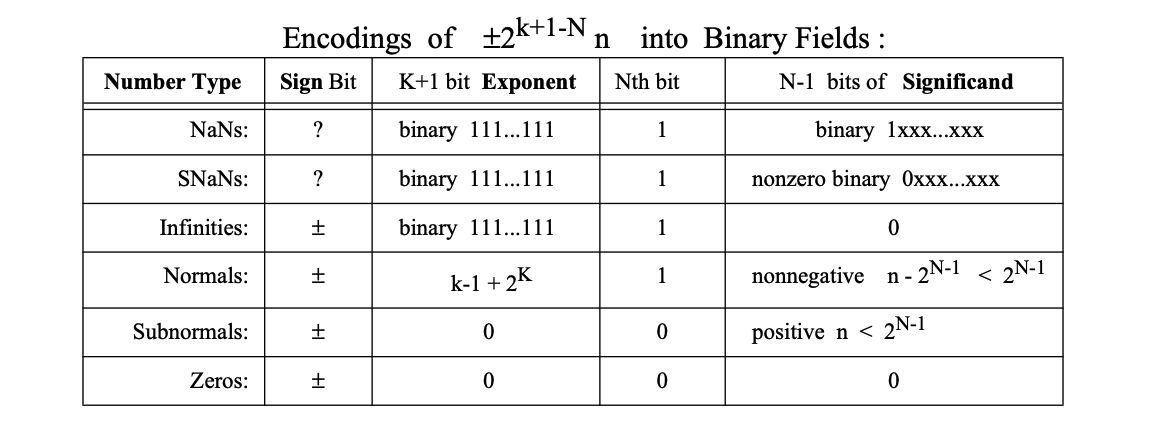
\includegraphics[width=1.0\textwidth]{pictures/inf_and_nan.png}
  \caption{IEEE754 float 定义 \label{fig:scatter}}
\end{figure}

\section{PyFloatObject}

\begin{lstlisting}[language=C, numbers=left, numbersep=1em, numberstyle=\footnotesize , breaklines=true]
// Include/floatobject.h
typedef struct {
    PyObject_HEAD
    double ob_fval;
} PyFloatObject;
\end{lstlisting}

PyFloatObject 对象的定义如上,PyObject\_HEAD 字段是大小不可变的 Python object 的统一头部,
ob\_fval 字段则是存储的 float 对象实际的值。为什么可以肯定的说 ob\_fval 存储的值就是 float 对象实际的值呢? 
我们可以通过一个实验来证明。在 Python 中可以通过下面的代码可以创建一个 float 对象,也就是虚拟机中的一个 PyFloatObject 对象。

\begin{lstlisting}[language=bash, numbers=left, numbersep=1em, numberstyle=\footnotesize , breaklines=true]
>>> f = float(3.14)
\end{lstlisting}

通过跟踪堆栈,发现最后进入了如下 PyFloat\_FromDouble 这个创建 PyFloatObject 对象的函数,在这个函数中,double 类型的
数字 3.14 被赋值给了 ob\_fval。

\begin{lstlisting}[language=C, numbers=left, numbersep=1em, numberstyle=\footnotesize , breaklines=true]
// Objects/floatobject.c
PyObject *
PyFloat_FromDouble(double fval)
{
    struct _Py_float_state *state = get_float_state();
    PyFloatObject *op = state->free_list;
    if (op != NULL) {
#ifdef Py_DEBUG
        // PyFloat_FromDouble() must not be called after _PyFloat_Fini()
        assert(state->numfree != -1);
#endif
        state->free_list = (PyFloatObject *) Py_TYPE(op);
        state->numfree--;
    }
    else {
        op = PyObject_Malloc(sizeof(PyFloatObject));
        if (!op) {
            return PyErr_NoMemory();
        }
    }
    _PyObject_Init((PyObject*)op, &PyFloat_Type);
    // 通过单步调试,发现最后 3.14 被赋值给了 op->ob_fval
    // 由此我们断定 ob_fval 被用来保存浮点数对象的真实值
    op->ob_fval = fval;
    return (PyObject *) op;
}
\end{lstlisting}

\section{对象池机制}

Python 的内置对象属于使用的非常频繁的对象,为了避免频繁的创建和释放这些类型的对象,Python 为他们设计
了一个对象池的机制。以本章研究的 PyFloatObjet 对象为例,我们来研究一下 Python 是如何实现它的对象池机制的。
首先看一下 PyFloatObject 在什么时候会使用对象池。

\begin{lstlisting}[language=C, numbers=left, numbersep=1em, numberstyle=\footnotesize , breaklines=true]
// Objects/floatobject.c
PyObject *
PyFloat_FromDouble(double fval)
{
    struct _Py_float_state *state = get_float_state();
    // [1] 获取对象池中的元素
    PyFloatObject *op = state->free_list;
    if (op != NULL) {
#ifdef Py_DEBUG
        // PyFloat_FromDouble() must not be called after _PyFloat_Fini()
        assert(state->numfree != -1);
#endif
	  // [2] 如果从空闲链表中获取到了元素,则需要将获取到的元素的
	  // 类型转换为 PyFloatObject
        state->free_list = (PyFloatObject *) Py_TYPE(op);
        // [3] 空闲链表上的元素数量减少1
        state->numfree--;
    }
    else {
        // [4] 空闲链表上没有元素了,则按照正常流程进行申请内存分配
        op = PyObject_Malloc(sizeof(PyFloatObject));
        if (!op) {
            return PyErr_NoMemory();
        }
    }
    // [5] 对获取到的对象进行初始化
    _PyObject_Init((PyObject*)op, &PyFloat_Type);
    op->ob_fval = fval;
    return (PyObject *) op;
}

\end{lstlisting}

PyFloat\_FromDouble 函数中的 state->free\_list 就是我们说的对象池了(虽说是对象池,但是叫做空闲对象链表更加合适一点)。 
可以看到流程是先调用 get\_float\_state 函数获取 struct \_Py\_float\_state* 类型的指针指向的一个 \_Py\_float\_state 实例 state,再
获取 state 上的 free\_list 作为我们需要的 PyFloatObject 对象。可以在这里没有到把这个元素从链表中取出的操作,也没有看到明显的对
链表的维护代码,难道这个叫做 free\_list 的东西只含有一个元素吗,那它为什么被叫做 list 呢?别着急,通过下面的分析,我们马上就可以
知道这些问题的答案了。不过我们还是先回到上面的代码,看一下如果没有从空闲链表中拿到元素,要怎么处理。从代码中的 [4] 处可
以看到,如果空闲链表中没有空闲的元素了,那么会走一个正常的申请内存分配的流程。不管是从空闲链表获取到的元素,还是通过
内存分配获取到的元素,在 [5] 处都要进行  PyFloatObject 对象的初始化。初始化的细节稍后再分析,我们下面回到空闲链表的话题。

先看一下持有了 free\_list 的家伙 \_Py\_float\_state 是什么一个构造。

\begin{lstlisting}[language=C, numbers=left, numbersep=1em, numberstyle=\footnotesize , breaklines=true]
struct _Py_float_state {
    /* Special free list
       free_list is a singly-linked list of available PyFloatObjects,
       linked via abuse of their ob_type members. */
    int numfree;
    PyFloatObject *free_list;
};
\end{lstlisting}

它的实现非常之简单,一个 numfree 成员表示空闲链表上元素的数量。还有一个 free\_list 指针。这个指针就是串联空闲链表的元素吗,
为什么看不到我们一般实现链表时候的 prev,next 指针呢,在上面的分析中,PyFloatObject 对象上可不存在这两个家伙。答案就藏在代码
的注释中,free\_list 通过利用 PyFloatObject 的 ob\_type 成员来链接链表上的元素。看起来很不可以思议,但其实都在情理之中,首先
空闲链表上的元素不需要 ob\_type 成员来表明类型,所以 ob\_type 可以被用作其他目的,例如这里的把空闲元素串连起来。其次,如果
需要按照标准的做法,使用一个 next 指针保存空闲链表的下一个元素,就需要在实现中多添加一个指针的大小,仅仅为了这个目的就增加
PyFloatObject 的内存大小,明显是得不偿失的,PyFloatObject 对象这种在运行时会大量创建的简单对象,每一个成员的添加都需要精打细算,避免造成过多的内存占用。从这两点看,使用 ob\_type 来链接空闲对象就很合理了。

清楚了空闲链表是如何串连起来的,接着研究一下我们上面提出的问题:空闲链表上的元素是如何被取下来的?
回到函数 PyFloat\_FromDouble。

\begin{lstlisting}[language=C, numbers=left, numbersep=1em, numberstyle=\footnotesize , breaklines=true]
PyObject *
PyFloat_FromDouble(double fval)
{
   // ... ...
    if (op != NULL) {
	  // ... ...
	  // [1] free_list 在这里指向了空闲链表中的下一个元素
        state->free_list = (PyFloatObject *) Py_TYPE(op);
        state->numfree--;
    }
	// ... ...
}

#define _PyObject_CAST(op) ((PyObject*)(op))

// [2] 返回的是 ob->ob_type
#define Py_TYPE(ob)             (_PyObject_CAST(ob)->ob_type)
\end{lstlisting}

看到上面的代码是不是恍然大悟了?在 [1] 处 free\_list 其实被赋予了一个新的值,这个新的值就是 [2] 处返回的当前 free\_list 首
元素的 ob\_type,在空闲链表的语境下,ob\_type 代表的就是空闲链表首个元素的下一个元素!

% 此处分析一下元素是如何添加到空闲链表的
知道了元素如何从空闲链表上取下来,那么我们一定也想知道元素是如何被添加到空闲链表上的。要了解这一点,可以从观察
PyFloatObject 对象 是如何被释放入手。

\begin{lstlisting}[language=C, numbers=left, numbersep=1em, numberstyle=\footnotesize , breaklines=true]
// Objects/floatobject.c

#  define PyFloat_MAXFREELIST   100

static void
float_dealloc(PyFloatObject *op)
{
    if (PyFloat_CheckExact(op)) {
        struct _Py_float_state *state = get_float_state();
#ifdef Py_DEBUG
        // float_dealloc() must not be called after _PyFloat_Fini()
        assert(state->numfree != -1);
#endif
	  // [1] 空闲链表达到上限,元素直接释放
        if (state->numfree >= PyFloat_MAXFREELIST)  {
            PyObject_Free(op);
            return;
        }
        // [2] 空闲链表没有达到上限,元素添加到空闲链表
        state->numfree++;
        Py_SET_TYPE(op, (PyTypeObject *)state->free_list);
        // [3] 要释放的元素变成了新的空闲链表头节点
        state->free_list = op;
    }
    else {
        Py_TYPE(op)->tp_free((PyObject *)op);
    }
}

// Include/object.h

// [4] 实际上就是 op->ob_type == state->free_list
static inline void _Py_SET_TYPE(PyObject *ob, PyTypeObject *type) {
    ob->ob_type = type;
}
#define Py_SET_TYPE(ob, type) _Py_SET_TYPE(_PyObject_CAST(ob), type)
\end{lstlisting}

从 [1] 处知道,如果空闲链表中连接的空闲元素数量达到了上限(当前版本中上限被定义为 100),那么就会将待释放的
元素直接释放。如果没有达到上限,才会考虑添加到空闲链表中。 [2] 处代码中调用了 Py\_SET\_TYPE 宏,而这个宏的
两个参数恰恰就是要释放的元素和空闲链表的头节点。结合 [3]、 [4] 两处的代码我们知道了,空闲链表的头节点成了
要释放元素 op 的下一个节点,op 变成了新的空闲链表头节点。

% 此处分析一下空闲链表是被谁管理的

了解清楚了空闲链表的机制,现在考虑新的问题:空闲链表是被谁管理的?多线程环境中空闲链表是怎么处理的?
带着这些问题,我们继续研究代码。get\_float\_state 函数作为获取 state 的入口,看一下它的内部实现。

\begin{lstlisting}[language=C, numbers=left, numbersep=1em, numberstyle=\footnotesize , breaklines=true]
// Objects/floatobject.c
static struct _Py_float_state *
get_float_state(void)
{
    // [1] 获取当前线程的解释器状态
    PyInterpreterState *interp = _PyInterpreterState_GET();
    return &interp->float_state;
}

// Include/internal/pycore_pystate.h
/* Get the current interpreter state.
   The macro is unsafe: it does not check for error and it can return NULL.
   The caller must hold the GIL.
   See also _PyInterpreterState_Get()
   and _PyGILState_GetInterpreterStateUnsafe(). */
static inline PyInterpreterState* _PyInterpreterState_GET(void) {
	// [2] 可以看到,这个 tstate 是每个线程都有一个的
    PyThreadState *tstate = _PyThreadState_GET();
#ifdef Py_DEBUG
    _Py_EnsureTstateNotNULL(tstate);
#endif
    return tstate->interp;
}
\end{lstlisting}

在 [1] 处代码可以看出,我们获取的 state 其实是一个 PyInterpreterState 的指针。看一下 PyInterpreterState 的定义。

\begin{lstlisting}[language=C, numbers=left, numbersep=1em, numberstyle=\footnotesize , breaklines=true]
// Include/pystate.h
typedef struct _is PyInterpreterState;

// Include/internal/pycore_interp.h
struct _is {
	// ... ...
	
   // 小整数池
    PyLongObject* small_ints[_PY_NSMALLNEGINTS + _PY_NSMALLPOSINTS];
    struct _Py_bytes_state bytes;
    struct _Py_unicode_state unicode;
    // PyFloatObject 空闲链表管理器
    struct _Py_float_state float_state;
    /* Using a cache is very effective since typically only a single slice is
       created and then deleted again. */
    PySliceObject *slice_cache;

    struct _Py_tuple_state tuple;
    struct _Py_list_state list;
    struct _Py_dict_state dict_state;
    struct _Py_frame_state frame;
    struct _Py_async_gen_state async_gen;
    struct _Py_context_state context;
    struct _Py_exc_state exc_state;
   // ... ...
};
\end{lstlisting}

可以看到,PyInterpreterState 这个结构不仅含有一个 PyFloatObject 空闲链表管理器,对其他多种 Python 内置对象,如 tuple,dict,int 等
都设置有对应的缓存机制。并且 PyInterpreterState 表示进程对象,Python 通过这个结构来模拟一个操作系统的进程,Python 的每个进程对应一个 PyInterpreterState 结构体。现在可以回答第一个问题了,空闲链表是被 PyInterpreterState 管理的。

回到上面的代码中,在摘抄代码时,我们特意留下了\_PyInterpreterState\_GET 函数的注释,注释中说到这个函数是不安全的,调用者
在调用这个函数的时候必须持有 GIL。而我们知道,这个 GIL 就是Python 中排他性的一个锁,每个线程要运行,就必须获得这把锁,所以
在调用 \_PyInterpreterState\_GET 时,必定只有一个线程能访问 PyInterpreterState,也就是说,空闲链表不会同时被 2 个及以上的线程访问,这也就可以回答前面提出的第二个问题:Python 通过 GIL 避免了多个线程同时访问空闲链表。

\begin{definition}[Python 对 GIL 的解释] \label{def:int}
  Notes about the implementation:

   - The GIL is just a boolean variable (locked) whose access is protected
     by a mutex (gil\_mutex), and whose changes are signalled by a condition
     variable (gil\_cond). gil\_mutex is taken for short periods of time,
     and therefore mostly uncontended.

   - In the GIL-holding thread, the main loop (PyEval\_EvalFrameEx) must be
     able to release the GIL on demand by another thread. A volatile boolean
     variable (gil\_drop\_request) is used for that purpose, which is checked
     at every turn of the eval loop. That variable is set after a wait of
     `interval` microseconds on `gil\_cond` has timed out.

      [Actually, another volatile boolean variable (eval\_breaker) is used
       which ORs several conditions into one. Volatile booleans are
       sufficient as inter-thread signalling means since Python is run
       on cache-coherent architectures only.]

   - A thread wanting to take the GIL will first let pass a given amount of
     time (`interval` microseconds) before setting gil\_drop\_request. This
     encourages a defined switching period, but doesn't enforce it since
     opcodes can take an arbitrary time to execute.

     The `interval` value is available for the user to read and modify
     using the Python API `sys.{get,set}switchinterval()`.

   - When a thread releases the GIL and gil\_drop\_request is set, that thread
     ensures that another GIL-awaiting thread gets scheduled.
     It does so by waiting on a condition variable (switch\_cond) until
     the value of last\_holder is changed to something else than its
     own thread state pointer, indicating that another thread was able to
     take the GIL.

     This is meant to prohibit the latency-adverse behaviour on multi-core
     machines where one thread would speculatively release the GIL, but still
     run and end up being the first to re-acquire it, making the "timeslices"
     much longer than expected.
     (Note: this mechanism is enabled with FORCE\_SWITCHING above)
\end{definition}


\section{参考资料}

\begin{itemize}
\item \href{https://peps.python.org/pep-3101/}{PEP 3101 – Advanced String Formatting}
\item \href{http://li.mit.edu/Archive/Activities/Archive/CourseWork/Ju_Li/MITCourses/18.335/Doc/IEEE754/ieee754.pdf}{IEEE Standard 754 for Binary Floating-Point Arithmetic}
\end{itemize}


 % Python 浮点数对象
%%%%%%%%%%%%%%%%%%%%%%%%%%%%%%%%%%%%%%%%%%%%%%%%%%%%%%%%%
%%%  整数对象
%%%%%%%%%%%%%%%%%%%%%%%%%%%%%%%%%%%%%%%%%%%%%%%%%%%%%%%%%
\chapter{Python 整数对象}
在 Python2 和 Python3 两个大版本中,对整数的内部实现发生了比较大的变化,在 Python2 中,整数分为两
类,PyIntObject 和 PyLongObject,但是在 Python3 中,整数对象完全由 PyLongObject 来实现,抛弃了
PyIntObject。Python3 中的整数对象定义在文件 longobject.h 中,由 PyLongObject 来实现,先来看一下它的具体定义。

\begin{lstlisting}[language=C, numbers=left, numbersep=1em, numberstyle=\footnotesize , breaklines=true]
// Include/longobject.h
typedef struct _longobject PyLongObject; 

// Include/longintrepr.h
struct _longobject {
    PyObject_VAR_HEAD
    digit ob_digit[1];
};
\end{lstlisting}

实现非常的简单,PyObject\_VAR\_HEAD 表示 PyLongObject 是一个变长对象,大小不是固定的,这个很容易推理,
我们知道,Python 的整数大小几乎是没有上限的,Python 又是使用 C 来实现,C 中没有任何一个基本类型可以放下
一个无限大小的整数,所以,Python 整数必然是使用一个变长对象来实现。把上面的 \_longobject 定义中的宏进行展开。

\begin{lstlisting}[language=C, numbers=left, numbersep=1em, numberstyle=\footnotesize , breaklines=true]
struct _longobject {
	struct {
    		PyObject ob_base;
    		Py_ssize_t ob_size;
	} PyVarObject;
    digit ob_digit[1];
};
\end{lstlisting}

其中的 digit 就是 uint32\_t 的别名。

\begin{figure}[htbp]
\centering
  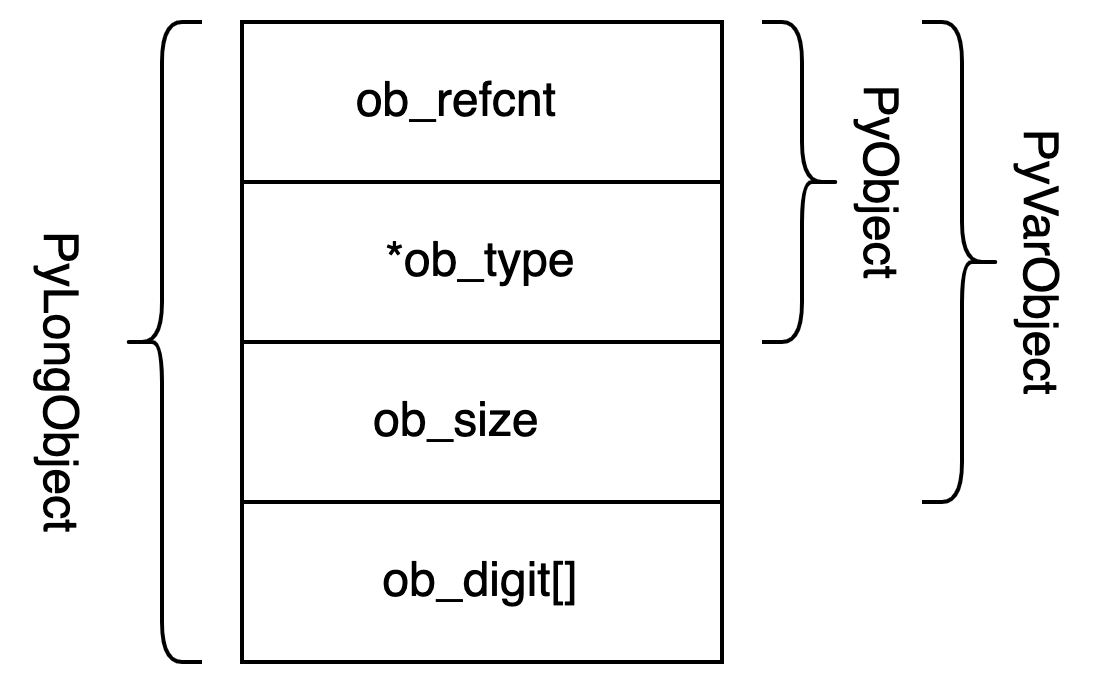
\includegraphics[width=0.5\textwidth]{pictures/ch5_01.png}
  \caption{PyLongObject 的结构 \label{fig:scatter}}
\end{figure}

在这个结构中,很容易看出可变的部分就是指 ob\_digit 数组。根据 \_longobject 结构体的注释,我们可以很轻松地
了解在 Python 中一个整数是怎么样表示的,下面我使用伪代码进行表示。

\begin{algorithm}
\caption{Python 中整数的表示}
$val = 0$\;
\If{$ob\_size == 0$}{
	\Return{0}\;
}
\For{$i \leftarrow 0$ \KwTo $\left|ob\_size \right| - 1$}{
	$val = val + ob\_digit\left[ i \right] \times 2^{SHIFT \times i}$\;
}
\If{$ob\_size > 0$}{
	\Return{$val$}\;
}
\Else{
	\Return{$-val$}
}
\end{algorithm}

算法还是简单易懂的,ob\_size 表示的是整数的符号和 ob\_digit 数组的大小。如果 ob\_size 等于 0 的话那么整数
值就是 0,如果 ob\_size 不等于 0,那么整数的符号就是 ob\_size 的符号,整数的绝对值就等于通过 ob\_digit 计算出来
的值。ob\_digit 的计算规则稍微复杂一点,所以我们通过例子来进行讲解。首先要说明一下伪代码中 SHIFT 这个值的含义。

在 Python 中,有一个叫做 PYLONG\_BITS\_IN\_DIGIT 的宏,表示 Python 整数对象中的 ob\_digit 数组的每个元素使用
的字节长度,如果 PYLONG\_BITS\_IN\_DIGIT 等于 30,那么 ob\_digit 数组就是一个 uint32\_t 数组,每个数组元素的
长度为 4 字节(32 位),如果 PYLONG\_BITS\_IN\_DIGIT 等于 15,那么 ob\_digit 数组就是一个 unsigned short 数组,每个数组
元素的长度为 2 字节(16 位)。PYLONG\_BITS\_IN\_DIGIT 的值表示 PyLongObject 使用 ob\_digit 数组成员的位数。
如果是uint32\_t 数组,那么对数组中的每个元素,只使用其中的 30 位,如果是 unsigned short 数组,对于数组中的每个成员,
只使用其中的 15 位。空出来的几位的作用是什么,下面会讲到。有两种定义的原因是考虑到不同机器的 int 长度不一样,
在 32 位机器喜爱,int 的长度是 2 字节,在 64 位机器下,int 的长度是 4 字节,需要针对不同的硬件做不同的调整。下面
的介绍中,如果没有特殊说明,默认 PYLONG\_BITS\_IN\_DIGIT 的值为 30。

现在可以告诉你了,上面伪代码中的 SHIFT 就是 PYLONG\_BITS\_IN\_DIGIT。现在有如下几个 PyLongObject 对象,来
计算一下它们表示的整数值。

\begin{figure}[htbp]
\centering
  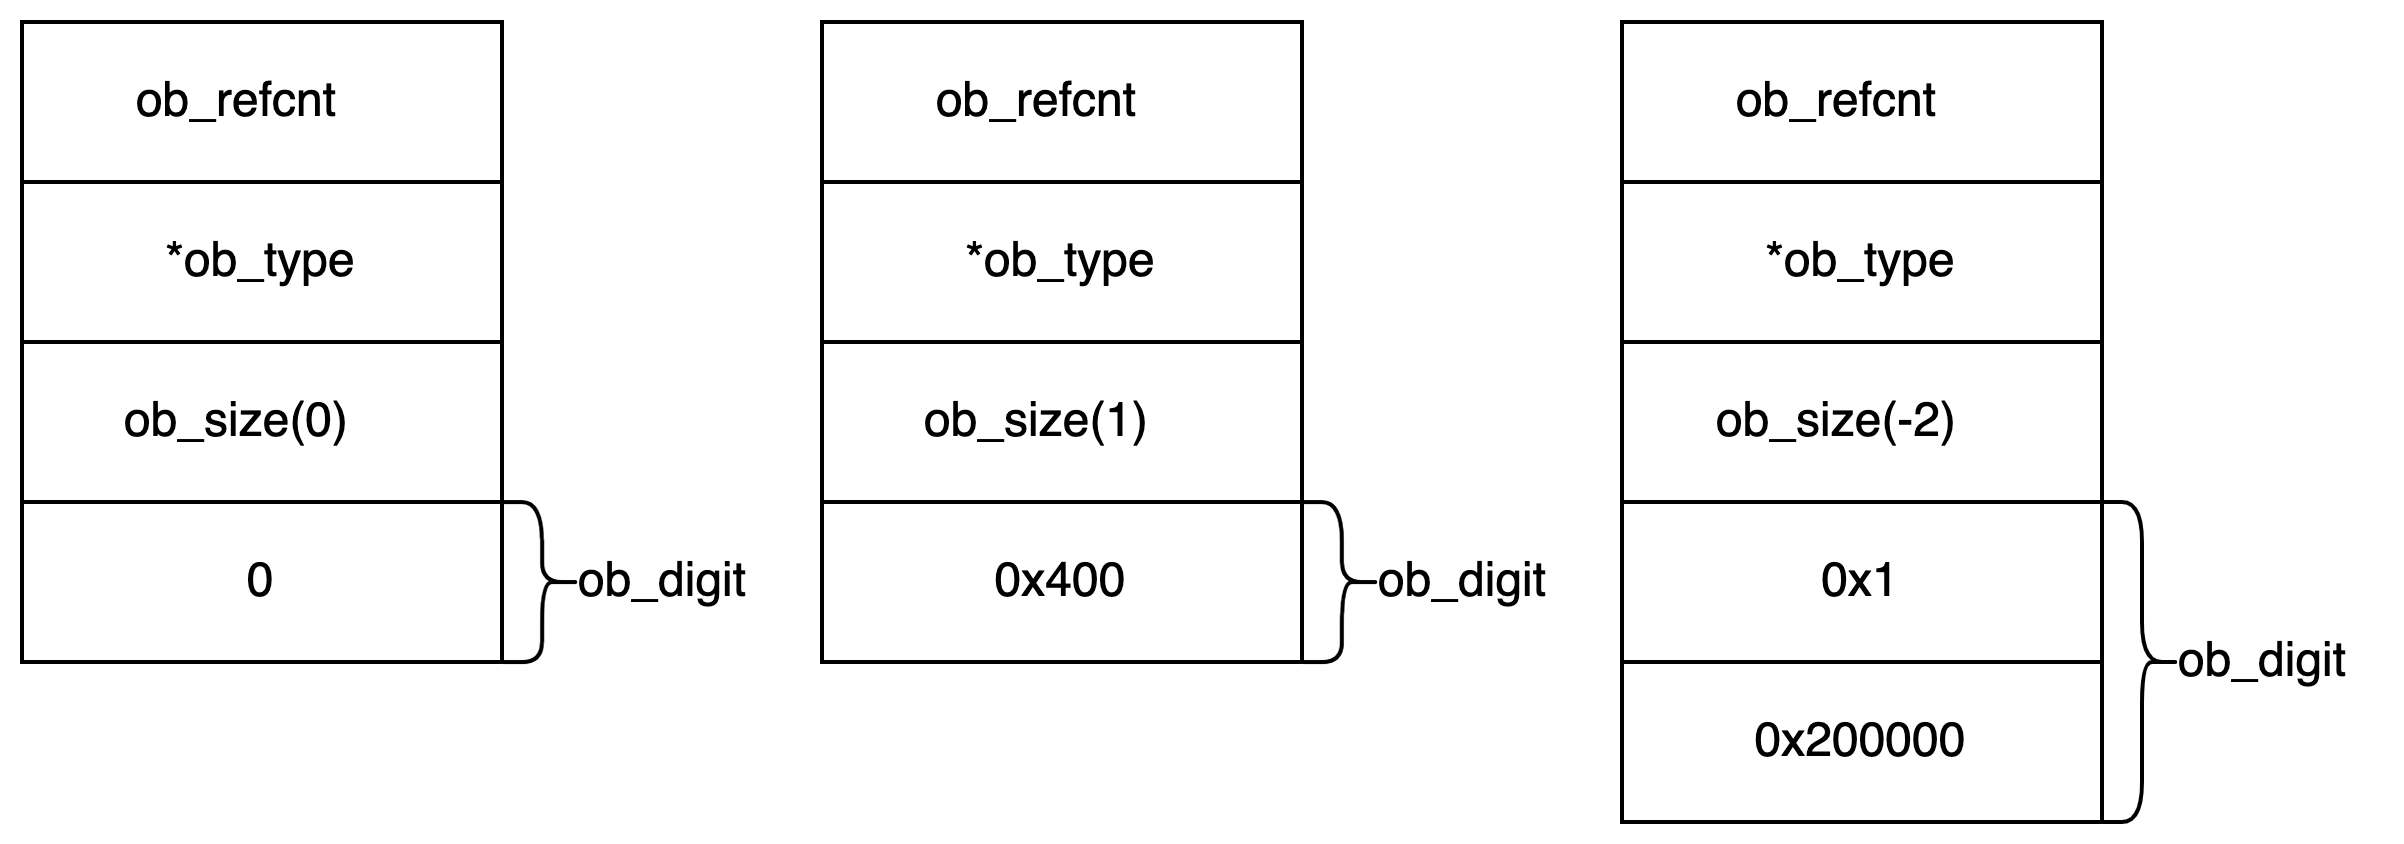
\includegraphics[width=0.8\textwidth]{pictures/ch5_02.png}
  \caption{3 个 PyLongObject 例子 \label{fig:scatter}}
\end{figure}

第一个 PyLongObject 中 ob\_size 等于 0,所以它表示的整数值就是 0 了。第二个 PyLongObject 中 ob\_size 等于 1,所以表示
的是一个正整数,ob\_size 等于 1 也说明 ob\_digit 数组的长度为 1,所以这个整数的值就是 0x400,也就是10进制整数 1024。
第三个 PyLongObject 中 ob\_size 等于 -2,说明这是一个负整数,并且 ob\_digit 数组的长度等于 2,根据 ob\_digit 数组和上面
伪代码给出的公式,算出整数的绝对值等于 $0x1 + 0x200000 \times 2^{30} = 2251799813685249$,所以第三个 PyLongObject 表示的整数
值就是 -2251799813685249。

下面是编写的2个函数,分别用来将一个整数转化为 ob\_size 和 ob\_digit,或者将 ob\_size 和 ob\_digit 转化为整数。
可以利用这组函数来验证上面对 PyLongObject 中整数值计算方法的描述。

\begin{lstlisting}[language=Python, numbers=left, numbersep=1em, numberstyle=\footnotesize , breaklines=true]
def int_2_digits(n:int):
    mod = 2**30
    flag = 1 if n >= 0 else -1
    ob_size = 0
    digits = []
    n = abs(n)
    
    while n > 0:
        digits.append(n % mod)
        n = n // mod
        ob_size += 1

    ob_size = flag * ob_size
    return ob_size, digits

def digits_2_int(ob_size:int, digits:list):
    SHIFT = 30
    n = 0
    if ob_size == 0:
        return n

    for i in range(abs(ob_size)):
        n += digits[i] * (2 ** (SHIFT * i))

    return n if ob_size > 0 else -n

def print_digits(n:int):
    ob_size, digits = int_2_digits(n)
    new_n = digits_2_int(ob_size, digits)
    digits = [hex(i) for i in digits]
    print("n:{} ob_size:{} digits:{} new_n:{}".format(n, ob_size, digits, new_n))
    assert n == new_n, "n:{} ob_size:{} digits:{} new_n:{}".format(n, ob_size, digits, new_n)

# 测试例子
print_digits(2**10)
print_digits(-(2**51+1))
\end{lstlisting}


\section{Python 中创建 PyLongObject 对象的几种方式}

Python 中,有多种方式可以创建一个 PyLongObject 对象,这些方式都定义在 longobject.h 文件中。

\begin{lstlisting}[language=C, numbers=left, numbersep=1em, numberstyle=\footnotesize , breaklines=true]
// Include/longobject.h
PyAPI_FUNC(PyObject *) PyLong_FromLong(long);
PyAPI_FUNC(PyObject *) PyLong_FromUnsignedLong(unsigned long);
PyAPI_FUNC(PyObject *) PyLong_FromSize_t(size_t);
PyAPI_FUNC(PyObject *) PyLong_FromSsize_t(Py_ssize_t);
PyAPI_FUNC(PyObject *) PyLong_FromDouble(double);
PyAPI_FUNC(PyObject *) PyLong_FromLongLong(long long);
PyAPI_FUNC(PyObject *) PyLong_FromUnsignedLongLong(unsigned long long);
// 省略掉其他一些
\end{lstlisting}

下面分析一下其中的几个例子。

\begin{lstlisting}[language=C, numbers=left, numbersep=1em, numberstyle=\footnotesize , breaklines=true]
// Objects/longobject.c
PyObject *
PyLong_FromLong(long ival)
{
    PyLongObject *v;
    // 保存 ival 的绝对值
    unsigned long abs_ival;
    unsigned long t;  /* unsigned so >> doesn't propagate sign bit */
    int ndigits = 0;
    int sign;
	// 如果是小整数那么直接返回小整数池中的对象
    if (IS_SMALL_INT(ival)) {
        return get_small_int((sdigit)ival);
    }
	// 如果 ival 是一个负数的话,是不可以通过取它的负数 -ival
	// 来获取绝对值,因为如果 ival = LONG_MIN 的话,-ival会溢出
    if (ival < 0) {
        abs_ival = 0U-(unsigned long)ival;
        sign = -1;
    }
    else {
        abs_ival = (unsigned long)ival;
        // 这里是一个亮点,记得上面提到过 ob_size 等于 0
        // 的话表示 PyLongObject 保存的整数值为 0 吗?
        sign = ival == 0 ? 0 : 1;
    }
    // 如果 ival 的绝对值使用一个 ob_digit 数组元素可以
    // 存下的话,那么进入快速通道
    if (!(abs_ival >> PyLong_SHIFT)) {
        v = _PyLong_New(1);
        if (v) {
            Py_SET_SIZE(v, sign);
            v->ob_digit[0] = Py_SAFE_DOWNCAST(
                abs_ival, unsigned long, digit);
        }
        return (PyObject*)v;
    }

// 如果 PyLong_SHIFT == 15 并且 abs_ival 可以使用两个 ob_digit 数组元素存下的话
// 则进行处理,类似上面的快速通道
#if PyLong_SHIFT==15
    /* 2 digits */
    if (!(abs_ival >> 2*PyLong_SHIFT)) {
        v = _PyLong_New(2);
        if (v) {
            Py_SET_SIZE(v, 2 * sign);
            v->ob_digit[0] = Py_SAFE_DOWNCAST(
                abs_ival & PyLong_MASK, unsigned long, digit);
            v->ob_digit[1] = Py_SAFE_DOWNCAST(
                  abs_ival >> PyLong_SHIFT, unsigned long, digit);
        }
        return (PyObject*)v;
    }
#endif

    // 这一步计算需要使用多少个元素的 ob_digit 数组可以放在这个整数
    t = abs_ival;
    while (t) {
        ++ndigits;
        t >>= PyLong_SHIFT;
    }
    v = _PyLong_New(ndigits);
    if (v != NULL) {
        digit *p = v->ob_digit;
        Py_SET_SIZE(v, ndigits * sign);
        t = abs_ival;
        // 对 PyLongObject 的 ob_digit 数组进行赋值
        while (t) {
            *p++ = Py_SAFE_DOWNCAST(
                t & PyLong_MASK, unsigned long, digit);
            t >>= PyLong_SHIFT;
        }
    }
    return (PyObject *)v;
}
\end{lstlisting}

上面的代码可以看出 PyLong\_FromLong 如何将一个 long 类型的整数转化为一个 PyLongObject 对象。
在 PyLong\_FromLong 函数里面,可以看到是使用 \_PyLong\_New 来创建一个 PyLongObject 对象,并且
给这个函数传递一个表示 ob\_digit 数组大小的参数。下面看看在它的内部究竟是做了什么操作才构造出
了一个 PyLongObject 对象。

\begin{lstlisting}[language=C, numbers=left, numbersep=1em, numberstyle=\footnotesize , breaklines=true]
// Objects/longobject.c
PyLongObject *
_PyLong_New(Py_ssize_t size)
{
    PyLongObject *result;
    // 如果申请的 ob_digit 数组的大小超过了 MAX_LONG_DIGITS,则抛出异常 
    if (size > (Py_ssize_t)MAX_LONG_DIGITS) {
        PyErr_SetString(PyExc_OverflowError,
                        "too many digits in integer");
        return NULL;
    }
    // 申请 PyLongObject 需要的内存大小
    result = PyObject_Malloc(offsetof(PyLongObject, ob_digit) +
                             size*sizeof(digit));
    if (!result) {
        PyErr_NoMemory();
        return NULL;
    }
    // 初始化 PyLongObject 对象
    _PyObject_InitVar((PyVarObject*)result, &PyLong_Type, size);
    return result;
}
\end{lstlisting}

\_PyLong\_New 函数的内容一目了然,主要包含两个步骤,申请内存和初始化 PyLongObject 对象。
在复制代码中时候,删除了关于申请内存处的一个注释,注释主要是说在之前的版本中,计算需要
申请的内存大小的方式是计算 sizeof(PyVarObject) + sizeof(digit)*size,但是在这个版本中使用的方式
是 offsetof(PyLongObject, ob\_digit) + sizeof(digit)*size,做这个改变的原因是在某些机器或者操作系统
中,使用 sizeof 计算可能会因为内存对齐导致计算的大小比实际的大小要大一些。为了验证这个说法,
下面写了一段简单的代码。

\begin{lstlisting}[language=C, numbers=left, numbersep=1em, numberstyle=\footnotesize , breaklines=true]
#include <stdio.h>
#include <stddef.h>
#include <stdint.h>

typedef ssize_t         Py_ssize_t;
typedef uint32_t digit;

typedef struct _object {
  Py_ssize_t ob_refcnt;
  void *ob_type; // 使用 void* 代替 PyTypeObject*
} PyObject;

typedef struct {
  PyObject ob_base;
  Py_ssize_t ob_size; /* Number of items in variable part */
} PyVarObject;

#define PyObject_VAR_HEAD      PyVarObject ob_base;

struct _longobject {
  PyObject_VAR_HEAD
  digit ob_digit[1];
};

typedef struct _longobject PyLongObject;

int main() {
  int n1 = sizeof(PyVarObject);
  int n2 = offsetof(PyLongObject, ob_digit);
  printf("n1=%d, n2=%d\n", n1, n2); /
  return 0;
}
\end{lstlisting}

但是在我的机器上输入结果是 $n1=24, n2=24$,两种计算方式并没有差异。
在在线编译器测试平台\\
 https://godbolt.org/ 上实验了多个编译器,也没有差异。
如果感兴趣的话,可以自己编译这一段代码试试看。

接下来继续看另一个创建 PyLongObject 对象的函数 PyLong\_FromDouble。这个函数中会用到 C
标准库中的 frexp 和 ldexp 函数,所以先对它进行一下介绍。frexp 函数的声明如下。

\begin{lstlisting}[language=C, numbers=left, numbersep=1em, numberstyle=\footnotesize , breaklines=true]
double frexp(double value, int *exp);

double ldexp(double x, int n);
\end{lstlisting}

frexp 函数会把浮点数参数 value 分解成为一个归一化的小数(就是frexp 函数的返回值,记做 ret,值的范围为 0 
和 $[\frac{1}{2}, 1)$)和 2 的整数幂(保存在 exp 中)。这两个数和 value 的关系是 $value = x \times 2^{exp} $。
ldexp 函数会计算 $ret = x \times 2^{n}$,其中 ret 是 ldexp 函数的返回值。了解了这个知识,继续看
PyLong\_FromDouble 函数吧。

\begin{lstlisting}[language=C, numbers=left, numbersep=1em, numberstyle=\footnotesize , breaklines=true]
PyObject *
PyLong_FromDouble(double dval)
{
    // 如果dval 的值在 long 的范围之内,调用 PyLong_FromLong 函数进行构造
    const double int_max = (unsigned long)LONG_MAX + 1;
    if (-int_max < dval && dval < int_max) {
        return PyLong_FromLong((long)dval);
    }

    PyLongObject *v;
    double frac;
    int i, ndig, expo, neg;
    neg = 0; // 表示是否是一个负数
    // 如果 dval 是 inf,抛出异常,返回 NULL
    if (Py_IS_INFINITY(dval)) {
        PyErr_SetString(PyExc_OverflowError,
                        "cannot convert float infinity to integer");
        return NULL;
    }
    // 如果 dval 是 nan,抛出异常,返回 NULL
    if (Py_IS_NAN(dval)) {
        PyErr_SetString(PyExc_ValueError,
                        "cannot convert float NaN to integer");
        return NULL;
    }
    if (dval < 0.0) {
        neg = 1;
        dval = -dval;
    }
    frac = frexp(dval, &expo); /* dval = frac*2**expo; 0.0 <= frac < 1.0 */
    assert(expo > 0);
    ndig = (expo-1) / PyLong_SHIFT + 1; /* Number of 'digits' in result */
    v = _PyLong_New(ndig);
    if (v == NULL)
        return NULL;
    frac = ldexp(frac, (expo-1) % PyLong_SHIFT + 1);
    for (i = ndig; --i >= 0; ) {
        digit bits = (digit)frac;
        v->ob_digit[i] = bits;
        frac = frac - (double)bits;
        frac = ldexp(frac, PyLong_SHIFT);
    }
    if (neg) {
        Py_SET_SIZE(v, -(Py_SIZE(v)));
    }
    return (PyObject *)v;
}
\end{lstlisting}

这个函数中比较难理解的部分是计算 ob\_digit 数组的值,将这一部分代码单独抽离出来看一下。

\begin{lstlisting}[language=C, numbers=left, numbersep=1em, numberstyle=\footnotesize , breaklines=true]
#include <stdio.h>
#include <math.h>
#include <inttypes.h>

#define PyLong_SHIFT 30
typedef uint32_t digit;

int main() {
  double dval = 6.917529027641082e+17; // 0.6 * 2**60
  double frac;
  int i, ndig, expo;

  frac = frexp(dval, &expo);
  // 计算出要用多少个 ob_digit 数组元素才可以保存下 double 的整数部分
  ndig = (expo-1) / PyLong_SHIFT + 1;
  frac = ldexp(frac, (expo-1) % PyLong_SHIFT + 1);
  for (i = ndig; --i >= 0;) { // 对 ob_digit 数组从高位到低位赋值
    digit bits = (digit)frac; // bits 就是 frac 的整数部分
    printf("%u ", bits);
    frac = frac - (double)bits; // frac 等于原来的 frac 的小数部分
    frac = ldexp(frac, PyLong_SHIFT); // frac = frac * 2**30
  }
  printf("\n");

  return 0;
}
\end{lstlisting}

编译执行上面这个 C 程序的输出如下。
\begin{lstlisting}[language=bash, numbers=left, numbersep=1em, numberstyle=\footnotesize , breaklines=true]
644245094 429496704
\end{lstlisting}

ob\_digit[1] = 644245094, ob\_digit[0] = 429496704。

PyLong\_FromDouble 函数之所以要如此大费周张的使用 frexp, ldexp 函数来进行计算,原因其实很简单:C 语言中没有任何一种整数
类型可以存储的下 double 的所有可能值整数部分,这样子是不是一下子就理解了。


\subsection{小整数池}

前面在快速通道的地方提到了小整数池,那么这一节就继续探究一下小整数池的内容。

\begin{lstlisting}[language=C, numbers=left, numbersep=1em, numberstyle=\footnotesize , breaklines=true]
#define _PY_NSMALLPOSINTS           257
#define _PY_NSMALLNEGINTS           5

#define NSMALLNEGINTS           _PY_NSMALLNEGINTS
#define NSMALLPOSINTS           _PY_NSMALLPOSINTS

#define IS_SMALL_INT(ival) (-NSMALLNEGINTS <= (ival) && (ival) < NSMALLPOSINTS)

PyObject *
PyLong_FromLong(long ival)
{
	// ... ...
    if (IS_SMALL_INT(ival)) {
        return get_small_int((sdigit)ival);
    }
    // ... ...
}
\end{lstlisting}

IS\_SMALL\_INT 宏用来判断一个整数是不是小整数,小整数的范围是 $[-5,\ 257)$。如果一个整数
在这个范围内的话,那么 PyLong\_FromLong 函数就会调用 get\_small\_int 函数来返回一个 PyLongObject。

\begin{lstlisting}[language=C, numbers=left, numbersep=1em, numberstyle=\footnotesize , breaklines=true]
// Objects/longobject.c
static PyObject *
get_small_int(sdigit ival)
{
    assert(IS_SMALL_INT(ival));
    PyObject *v = __PyLong_GetSmallInt_internal(ival);
    Py_INCREF(v);
    return v;
}

static inline PyObject* __PyLong_GetSmallInt_internal(int value)
{
    PyInterpreterState *interp = _PyInterpreterState_GET();
    assert(-_PY_NSMALLNEGINTS <= value && value < _PY_NSMALLPOSINTS);
    size_t index = _PY_NSMALLNEGINTS + value;
    // 直接从 interp->small_ints 数组中获取缓存的 PyLongObject 对象
    PyObject *obj = (PyObject*)interp->small_ints[index];
    assert(obj != NULL);
    return obj;
}

\end{lstlisting}

interp->small\_ints 的初始化是在 \_PyLong\_Init 中实现的,可以看到其中使用一个 for 循环,生成了 5 + 257 个 PyLongObject
对象保存在 small\_ints 数组中。

\begin{lstlisting}[language=C, numbers=left, numbersep=1em, numberstyle=\footnotesize , breaklines=true]
int
_PyLong_Init(PyInterpreterState *interp)
{
    for (Py_ssize_t i=0; i < NSMALLNEGINTS + NSMALLPOSINTS; i++) {
        sdigit ival = (sdigit)i - NSMALLNEGINTS;
        int size = (ival < 0) ? -1 : ((ival == 0) ? 0 : 1);

        PyLongObject *v = _PyLong_New(1);
        if (!v) {
            return -1;
        }

        Py_SET_SIZE(v, size);
        v->ob_digit[0] = (digit)abs(ival);

        interp->small_ints[i] = v;
    }
    return 0;
}
\end{lstlisting}




\section{参考资料}

\begin{itemize}
\item \href{https://flaggo.github.io/python3-source-code-analysis/objects/long-object/}{Python 整数对象}
\item \href{https://godbolt.org/}{Compiler Explorer}
\end{itemize}
 % Python 整数对象
%%%%%%%%%%%%%%%%%%%%%%%%%%%%%%%%%%%%%%%%%%%%%%%%%%%%%%%%%
%%%  字符串对象
%%%%%%%%%%%%%%%%%%%%%%%%%%%%%%%%%%%%%%%%%%%%%%%%%%%%%%%%%
\chapter{Python 字符串对象}

在 Python 3.3 之后,cpython 中 Unicode 字符串的内部表示发生了变化,Unicode 字符串有多个内部表示形式,具体
使用哪一种取决于字符串中最大的 Unicode 字符。具体规则如下:
\begin{itemize}
\item 如果字符串中所有的 Unicode 字符都可以使用一个字节表示,那么使用 Py\_UCS1,也即是 latin1 格式的内部表示。
\item 如果字符串中所有的 Unicode 字符都可以使用两个字节表示,那么使用 Py\_UCS2 格式的内部表示。
\item 如果字符串中所有的 Unicode 字符都可以使用四个字节表示,那么使用 Py\_UCS4 格式的内部表示。
\end{itemize}

在具体进行说明之前,先说明一下 Unicode,UCS 和字符之间的关系。Unicode 是为了给世界上各种字符一个唯一的表示而
设计的一种标准,任何字符在 Unicode 中都对应一个值,这个值被称为 code point。反过来说就是 code point 是指定 Unicode
系统中某个字符的一个数字。在 Unicode 系统中,code point 使用 "U+1234" 这样的形式进行表示,其中 1234 就代表这个 code
point 被分配的数字,例如,字符 "a" 被分配的 code point 是 "U+0041"。有了 code point,还需要具体的编码规则,将 code point
储存到计算机中,这个储存规则就是字符编码规则。UCSUCS-2 和 UCS-4 就是两种字符编码规则,分别使用 2 个字节和四个字节来编码
一个 Unicode 字符,很明显,如果 2 个字节就可以包括所有的 Unicode 字符,那么就完全不需要耗费双倍存储空间的 UCS-4 了,所以
UCS-2 表示的是完整的 Unicode 字符集的一个子集,使用 UCS-2 不能表示任意一个 Unicode 字符。常见的 UTF-16 就是一个 UCS-2 的
一个具体实现,UTF-32 就是一个 UCS-4 的具体实现。

回到 Python 中来,上面提到的 Python 会根据 Unicode 字符串中最大的 Unicode 字符来选择一个内部编码就很好理解了,
如果字符串是一个简单的 ASCII 字符串,那么使用每个字符一个字节的 latin1 编码最省存储空间,如果字符串中最大的字符可以使用
UCS-2 表示,那么使用每个字符占 2 个字节的 UCS-2 编码最省空间,如果字符串中最大的字符超过 UCS-2 能表示的范围,那么就使用
UCS-4 来编码字符串。

但是我们这个时候会有一个疑问,如果一个很长的字符串中除了一个需要用 UCS-4 表示的字符,其他全部都是 ASCII 字符串,那不是因为
这一个字符导致存储字符串需要的空间变大了接近 3 倍吗?使用一个变长字符的编码,对 ASCII 字符使用一个字节存储,对在 UCS-2 范围
内的字符使用 2 字节进行存储,对在 UCS-4 范围内的字符使用 3 或 4 字节进行存储,不是才最省空间吗。
是的,使用变长编码(例如 UTF-8)的字符串确实会比使用 UCS-2 和 UCS-4 省很多空间,在极端情况下甚至可以省 3/4,但是,使用变长
编码来存储字符串也是有代价的。可以考虑这个问题,如果一个字符串中,每个字符都使用 2 个字节进行表示,那么要快速访问第 N 个
字符,有一种非常简单的方式,就是 字符串首字符地址 + 2 * (N-1)。但是如果使用变长编码来存储字符串的话,要访问第 N 个字符,就
需要对字符串的每个字节进行遍历,依次解析出每个字符,这样子才可以确定第 N 个字符的位置。所以,Python 不采用变长编码是一种
空间换时间的做法。

Python 内部将字符串分成了 4 种。

第一种是紧凑的 ASCII 字符串,这种字符串使用 PyASCIIObject 来进行表示。它的类型为 PyUnicode\_1BYTE\_KIND。

第二种是紧凑的字符串,它使用 PyCompactUnicodeObject 表示。类型为 PyUnicode\_1BYTE\_KIND,PyUnicode\_2BYTE\_KIND
或者 PyUnicode\_4BYTE\_KIND。PyUnicode\_1BYTE\_KIND 这种类型的字符串是每个字符能用一个字节表示的字符串,也就是 latin1
字符串,ASCII 是 latin1 的子集,所以纯 ASCII 字符串使用第一种字符串来保存,纯 latin1 字符串就使用第二种字符串来保存。

第三种是旧版本,且 ready 状态为 0 的字符串,这种字符串使用 PyUnicodeObject 来表示。它的类型为 PyUnicode\_WCHAR\_KIND。

第四种是旧版本,且 ready 状态为 1 的字符串,使用 PyUnicodeObject 表示,类型为 PyUnicode\_1BYTE\_KIND,PyUnicode\_2BYTE\_KIND
或者 PyUnicode\_4BYTE\_KIND。

紧凑的字符串使用一块完整的内存来保存字符串需要的结构体和字符串内容。旧版本字符串则使用两块内存来保存,其中一块用来保存
字符串结构体,一块用来保存字符串内容,并且结构体中有一个指针指向第二个内存块。

旧版本的字符串使用 PyUnicode\_FromUnicode() 和 PyUnicode\_FromStringAndSize(NULL, size) 函数进行创建,并且在 PyUnicode\_READY()
函数被调用之后 ready 状态才由 0 变为 1。


下面看一个 Python3 中具体是如何实现字符串功能的。

\begin{lstlisting}[language=C, numbers=left, numbersep=1em, numberstyle=\footnotesize , breaklines=true]
typedef struct {
    PyObject_HEAD
    Py_ssize_t length;  // 字符串中代码点的数量,可以理解为符号数量
    Py_hash_t hash;
    struct {
        unsigned int interned:2; // 字符串是否被共享
        unsigned int kind:3;  // 字符串采用的编码方式
        unsigned int compact:1;  // 对象是否和文本内容一起分配
        unsigned int ascii:1;  // 字符串是否都是 ASCII 字符
        unsigned int ready:1; // 字符串对象是否初始化完成
        unsigned int :24;  // 用来做内存对齐
    } state;
    wchar_t *wstr;  // 指向宽字符数组的指针,数组以 "\0" 结尾
} PyASCIIObject;

typedef struct {
    PyASCIIObject _base;
    Py_ssize_t utf8_length;  // utf8 字符串中的字节数,不包括结尾的空字符
    char *utf8;                 // 指向 utf8字符数组的指针,字符数组以 \0 结尾
    Py_ssize_t wstr_length;    // wstr 中代码点的数量
                                 * surrogates count as two code points. */
} PyCompactUnicodeObject;

typedef struct {
    PyCompactUnicodeObject _base;
    union {
        void *any;
        Py_UCS1 *latin1;
        Py_UCS2 *ucs2;
        Py_UCS4 *ucs4;
    } data;                     /* Canonical, smallest-form Unicode buffer */
} PyUnicodeObject;
\end{lstlisting}

分析完了字符串的存储结构,接下来看一下 Python 中的字符串是如何创建的。

首先看一下旧版本字符串的创建函数 PyUnicode\_FromUnicode 和 PyUnicode\_FromStringAndSize。

\begin{lstlisting}[language=C, numbers=left, numbersep=1em, numberstyle=\footnotesize , breaklines=true]
PyObject *
PyUnicode_FromUnicode(const Py_UNICODE *u, Py_ssize_t size)
{
    // 如果字符串为空
    if (u == NULL) {
        if (size > 0) {
            if (PyErr_WarnEx(PyExc_DeprecationWarning,
                    "PyUnicode_FromUnicode(NULL, size) is deprecated; "
                    "use PyUnicode_New() instead", 1) < 0) {
                return NULL;
            }
        }
        // i == NULL 并且 size >= 0,返回调用 _PyUnicode_New 创建的字符串
        return (PyObject*)_PyUnicode_New(size);
    }
	// size < 0 抛出错误
    if (size < 0) {
        PyErr_BadInternalCall();
        return NULL;
    }
	// u != NULL 并且 size >= 0,返回 PyUnicode_FromWideChar 创建的字符串
    return PyUnicode_FromWideChar(u, size);
}
\end{lstlisting}

PyUnicode\_FromUnicode 其实内部也没有逻辑,最后还是调用 \_PyUnicode\_New 和 PyUnicode\_FromWideChar 来创建
PyUnicodeObject 对象。

\begin{lstlisting}[language=C, numbers=left, numbersep=1em, numberstyle=\footnotesize , breaklines=true]
static PyUnicodeObject *
_PyUnicode_New(Py_ssize_t length)
{
    PyUnicodeObject *unicode;
    size_t new_size;

    // [1] 如何 length 为 0,那么直接返回一个共享的空字符串
    if (length == 0) {
        return (PyUnicodeObject *)unicode_new_empty();
    }

    // 检查需要申请的字符串长度,如果太长,直接抛出错误
    if (length > ((PY_SSIZE_T_MAX / (Py_ssize_t)sizeof(Py_UNICODE)) - 1)) {
        return (PyUnicodeObject *)PyErr_NoMemory();
    }
    // length < 0 也是不合法的
    if (length < 0) {
        PyErr_SetString(PyExc_SystemError,
                        "Negative size passed to _PyUnicode_New");
        return NULL;
    }
    // 创建一个 PyUnicodeObject 结构
    unicode = PyObject_New(PyUnicodeObject, &PyUnicode_Type);
    if (unicode == NULL)
        return NULL;
    new_size = sizeof(Py_UNICODE) * ((size_t)length + 1);

    // PyUnicodeObject 一些数据结构的初始化
    _PyUnicode_WSTR_LENGTH(unicode) = length;
    _PyUnicode_HASH(unicode) = -1;
    _PyUnicode_STATE(unicode).interned = 0;
    _PyUnicode_STATE(unicode).kind = 0;
    _PyUnicode_STATE(unicode).compact = 0;
    // 注意,ready 是被初始化为 0 的
    _PyUnicode_STATE(unicode).ready = 0;
    _PyUnicode_STATE(unicode).ascii = 0;
    _PyUnicode_DATA_ANY(unicode) = NULL;
    _PyUnicode_LENGTH(unicode) = 0;
    _PyUnicode_UTF8(unicode) = NULL;
    _PyUnicode_UTF8_LENGTH(unicode) = 0;
    // 申请分配存储字符串需要的存储空间
    _PyUnicode_WSTR(unicode) = (Py_UNICODE*) PyObject_Malloc(new_size);
    if (!_PyUnicode_WSTR(unicode)) {
        Py_DECREF(unicode);
        PyErr_NoMemory();
        return NULL;
    }

   // 这里是为了避免 unicode_resize 读到未初始化的内存专门做的
    _PyUnicode_WSTR(unicode)[0] = 0;
    _PyUnicode_WSTR(unicode)[length] = 0;

    assert(_PyUnicode_CheckConsistency((PyObject *)unicode, 0));
    return unicode;
}
\end{lstlisting}

从代码中可以看到 \_PyUnicode\_New 函数中 unicode 结构体和 unicode->wstr 不是一次分配出来的,
这样验证了前面提到的 PyUnicodeObject 类型中结构体和字符串的实际数据是由两块内存保存的说法。

上面 [1] 处提到了如果申请创建的 Unicode 字符串长度为 0,那么会返回一个共享的空字符串,这是 Python 的一个优化,
公用一个空字符串可以节约部分内存,还可以避免字符串长度为 0 的 PyUnicodeObject 对象的创建和销毁成本,
下面看一下空字符串优化的实现细节。

\begin{lstlisting}[language=C, numbers=left, numbersep=1em, numberstyle=\footnotesize , breaklines=true]
// Return a strong reference to the empty string singleton.
static inline PyObject* unicode_new_empty(void)
{
    PyObject *empty = unicode_get_empty();
    Py_INCREF(empty);
    return empty;
}

// Return a borrowed reference to the empty string singleton.
static inline PyObject* unicode_get_empty(void)
{
    struct _Py_unicode_state *state = get_unicode_state();
    // unicode_get_empty() must not be called before _PyUnicode_Init()
    // or after _PyUnicode_Fini()
    assert(state->empty_string != NULL);
    return state->empty_string;
}

static struct _Py_unicode_state*
get_unicode_state(void)
{
    PyInterpreterState *interp = _PyInterpreterState_GET();
    return &interp->unicode;
}
\end{lstlisting}

可以看到,空字符串其实就是 PyInterpreterState 结构体中的 unicode 字段,和Python 整数实现章节中介绍的 interp->small\_ints 的初始化类似,
这个字段的初始化是通过 \_PyUnicode\_Init 进行的。

\begin{lstlisting}[language=C, numbers=left, numbersep=1em, numberstyle=\footnotesize , breaklines=true]
PyStatus
_PyUnicode_Init(PyInterpreterState *interp)
{
    struct _Py_unicode_state *state = &interp->unicode;
    // unicode_create_empty_string_singleton 函数对 unicode 进行初始化
    if (unicode_create_empty_string_singleton(state) < 0) {
        return _PyStatus_NO_MEMORY();
    }
    // 省略初始化布隆过滤器的代码
    return _PyStatus_OK();
}

static int
unicode_create_empty_string_singleton(struct _Py_unicode_state *state)
{
    // 创建对象的时候使用size 为 1 进行申请,这样子之后使用到 state->empty_string
    // 的地方就不需要检查是否为 NULL 了。
    PyObject *empty = PyUnicode_New(1, 0);
    if (empty == NULL) {
        return -1;
    }
    PyUnicode_1BYTE_DATA(empty)[0] = 0;
    _PyUnicode_LENGTH(empty) = 0;
    assert(_PyUnicode_CheckConsistency(empty, 1));

    assert(state->empty_string == NULL);
    state->empty_string = empty;
    return 0;
}
\end{lstlisting}

了解了空字符串优化,继续回到 PyUnicode\_FromUnicode 调用的的另一个创建函数 PyUnicode\_FromWideChar。

\begin{lstlisting}[language=C, numbers=left, numbersep=1em, numberstyle=\footnotesize , breaklines=true]
PyObject *
PyUnicode_FromWideChar(const wchar_t *u, Py_ssize_t size)
{
    PyObject *unicode;
    Py_UCS4 maxchar = 0;
    Py_ssize_t num_surrogates;

    if (u == NULL && size != 0) {
        PyErr_BadInternalCall();
        return NULL;
    }

    if (size == -1) {
        size = wcslen(u);
    }

    // 对空字符串返回共享的对象
    if (size == 0)
        _Py_RETURN_UNICODE_EMPTY();
    // 处理 Oracle Solaris 操作系统上的特例,略过

    // 处理单字节 latin1 字符
    if (size == 1 && (Py_UCS4)*u < 256)
        return get_latin1_char((unsigned char)*u);

    // 找出字符串中最大的字符存储在 maxchar, 求出最大 Unicode 字符的目的是为了确定这个 Unicode 字符串
    //可以转化为一个 UCS-1,UCS-2 还是一个 UCS-4 字符串
    // 如果系统的 wchar_t 是采用双字节(一个unicode z字符使用两个 wchar_t 存储), 那么 num_surrogates 表示
    // 使用两个存储双字节字符的个数。其实这里很容易理解,如果字符串数组 u 的 size 是 n,那么字符串中
    // 存储的 unicode 字符数就是 n - num_surrogates
    if (find_maxchar_surrogates(u, u + size,
                                &maxchar, &num_surrogates) == -1)
        return NULL;
    // 这里使用 size - num_surrogates 而不是 num_surrogates 来表示字符数目是因为 u 的末尾可能有一个空字符
    unicode = PyUnicode_New(size - num_surrogates, maxchar);
    if (!unicode)
        return NULL;
    // 将 Unicode 字符串 u 转化为 PyUnicode_1BYTE_KIND/PyUnicode_2BYTE_KIND/
    // PyUnicode_4BYTE_KIND 中的一种格式
    switch (PyUnicode_KIND(unicode)) {
    case PyUnicode_1BYTE_KIND:
        _PyUnicode_CONVERT_BYTES(Py_UNICODE, unsigned char,
                                u, u + size, PyUnicode_1BYTE_DATA(unicode));
        break;
    case PyUnicode_2BYTE_KIND:
#if Py_UNICODE_SIZE == 2
        memcpy(PyUnicode_2BYTE_DATA(unicode), u, size * 2);
#else
        _PyUnicode_CONVERT_BYTES(Py_UNICODE, Py_UCS2,
                                u, u + size, PyUnicode_2BYTE_DATA(unicode));
#endif
        break;
    case PyUnicode_4BYTE_KIND:
#if SIZEOF_WCHAR_T == 2
        unicode_convert_wchar_to_ucs4(u, u + size, unicode);
#else
        assert(num_surrogates == 0);
        memcpy(PyUnicode_4BYTE_DATA(unicode), u, size * 4);
#endif
        break;
    default:
        Py_UNREACHABLE();
    }
    return unicode_result(unicode);
}
\end{lstlisting}

可以看到 PyUnicode\_FromWideChar 的流程虽然很复杂,但是功能其实蛮清晰的,就是把一个用 wchar\_t 数组存储的 Unicode 字符串转化为
一个 PyUnicodeObject 对象。

下面接着分析 PyUnicode\_FromStringAndSize 函数的实现,PyUnicode\_FromStringAndSize 和 PyUnicode\_FromUnicode 函数
很类似,只是它的第一个参数 u 是一个 UTF-8 编码的字节数组。

\begin{definition}[UTF-8编码介绍] \label{def:int}
UTF-8 是 Unicode 编码的一种实现方式,它是一种变长的编码,使用 1 到 4 个字节来表示一个 Unicode 符号。Unicode 的编码规则如下:
\begin{itemize}
\item 对于单字节的符号,字节的第一位设为 0,后面 7 位为这个符号的 Unicode 码。因此对于英语字母,UTF-8 编码和 ASCII 码是相同的。
\item 对于 n 字节的符号(n > 1),第一个字节的前 n 位都设为 1,第 n + 1 位设为0,后面字节的前两位一律设为 10。剩下的没有提及的二进制位,全部为这个符号的 Unicode 码。
\end{itemize}
\end{definition}

\begin{lstlisting}[language=C, numbers=left, numbersep=1em, numberstyle=\footnotesize , breaklines=true]
PyObject *
PyUnicode_FromStringAndSize(const char *u, Py_ssize_t size)
{
    if (size < 0) {
        PyErr_SetString(PyExc_SystemError,
                        "Negative size passed to PyUnicode_FromStringAndSize");
        return NULL;
    }
    if (u != NULL) {
        // 如果字符数组不为空,那么将 UTF-8 编码的字符串转化为一个使用 UCS-1,UCS-2 
        // 或 UCS-4 编码的 PyUnicodeObject 对象
        return PyUnicode_DecodeUTF8Stateful(u, size, NULL, NULL);
    }
    else {
        if (size > 0) {
            if (PyErr_WarnEx(PyExc_DeprecationWarning,
                    "PyUnicode_FromStringAndSize(NULL, size) is deprecated; "
                    "use PyUnicode_New() instead", 1) < 0) {
                return NULL;
            }
        }
        return (PyObject *)_PyUnicode_New(size);
    }
}
\end{lstlisting}

上面介绍了 PyUnicodeObject 对象的两种创建方式,一种是 wchar\_t 字符数组转化为 PyUnicodeObject 对象,另一种是 UTF-8 
数组转化为 PyUnicodeObject 对象。下面回到基础的部分也是我们日常接触的最多的部分,也就是 PyASCIIObject 对象的创建。
创建 PyASCIIObject 的函数接口是 PyUnicode\_New。PyUnicode\_New 函数不仅仅用来创建 PyASCIIObject,事实上,在 PEP 393
之后,它就是创建一个 Unicode 对象最推荐的方式。PyUnicode\_New 会申请一整块内存用来存储 Unicode 对象和对应的字符串,
所以使用这个函数创建的 Unicode 对象都是不可以重新分配大小的。

\begin{lstlisting}[language=C, numbers=left, numbersep=1em, numberstyle=\footnotesize , breaklines=true]
PyObject *
PyUnicode_New(Py_ssize_t size, Py_UCS4 maxchar)
{
    // 空字符串优化
    if (size == 0) {
        return unicode_new_empty();
    }

    PyObject *obj;
    PyCompactUnicodeObject *unicode;
    void *data;
    enum PyUnicode_Kind kind;
    int is_sharing, is_ascii;
    Py_ssize_t char_size;
    Py_ssize_t struct_size;

    is_ascii = 0;
    is_sharing = 0;
    struct_size = sizeof(PyCompactUnicodeObject);
    if (maxchar < 128) {
        kind = PyUnicode_1BYTE_KIND;
        char_size = 1;
        is_ascii = 1;
        struct_size = sizeof(PyASCIIObject);
    }
    else if (maxchar < 256) {
        kind = PyUnicode_1BYTE_KIND;
        char_size = 1;
    }
    else if (maxchar < 65536) {
        kind = PyUnicode_2BYTE_KIND;
        char_size = 2;
        if (sizeof(wchar_t) == 2)
            is_sharing = 1;
    }
    else {
        if (maxchar > MAX_UNICODE) {
            PyErr_SetString(PyExc_SystemError,
                            "invalid maximum character passed to PyUnicode_New");
            return NULL;
        }
        kind = PyUnicode_4BYTE_KIND;
        char_size = 4;
        if (sizeof(wchar_t) == 4)
            is_sharing = 1;
    }

    // 处理 size 为负数或者超过最大值的情况
    if (size < 0) {
        PyErr_SetString(PyExc_SystemError,
                        "Negative size passed to PyUnicode_New");
        return NULL;
    }
    if (size > ((PY_SSIZE_T_MAX - struct_size) / char_size - 1))
        return PyErr_NoMemory();

    // 给 PyCompactUnicodeObject 结构体和字符数组申请空间
    obj = (PyObject *) PyObject_Malloc(struct_size + (size + 1) * char_size);
    if (obj == NULL) {
        return PyErr_NoMemory();
    }
    // 对象类型初始化
    _PyObject_Init(obj, &PyUnicode_Type);

    unicode = (PyCompactUnicodeObject *)obj;
    // 这里这个判断需要注意,如果保存的字符串都是 ASCII 字符,那么字符数组会被
    // 保存到 PyASCIIObject 结构体的最末尾位置
    // 如果不是纯 ASCII 字符串,那吗字符数组会被保存到 PyCompactUnicodeObject 结构体
    // 的最末尾位置,所以下面的代码其实就是就是在确定字符数组的地址
    if (is_ascii)
        data = ((PyASCIIObject*)obj) + 1;
    else
        data = unicode + 1;
    _PyUnicode_LENGTH(unicode) = size;
    _PyUnicode_HASH(unicode) = -1;
    _PyUnicode_STATE(unicode).interned = 0;
    _PyUnicode_STATE(unicode).kind = kind;
    _PyUnicode_STATE(unicode).compact = 1;
    _PyUnicode_STATE(unicode).ready = 1;
    _PyUnicode_STATE(unicode).ascii = is_ascii;
    // 字符数组末尾添加一个空字符并且将用不到的字符数组指针设置为空
    if (is_ascii) {
        ((char*)data)[size] = 0;
        _PyUnicode_WSTR(unicode) = NULL;
    }
    else if (kind == PyUnicode_1BYTE_KIND) {
        ((char*)data)[size] = 0;
        _PyUnicode_WSTR(unicode) = NULL;
        _PyUnicode_WSTR_LENGTH(unicode) = 0;
        unicode->utf8 = NULL;
        unicode->utf8_length = 0;
    }
    else {
        unicode->utf8 = NULL;
        unicode->utf8_length = 0;
        if (kind == PyUnicode_2BYTE_KIND)
            ((Py_UCS2*)data)[size] = 0;
        else /* kind == PyUnicode_4BYTE_KIND */
            ((Py_UCS4*)data)[size] = 0;
        // is_sharing 标记用来决定要不要给 unicode->wstr 指针赋值,也指向保存字符数组的位置
        if (is_sharing) {
            _PyUnicode_WSTR_LENGTH(unicode) = size;
            _PyUnicode_WSTR(unicode) = (wchar_t *)data;
        }
        else {
            _PyUnicode_WSTR_LENGTH(unicode) = 0;
            _PyUnicode_WSTR(unicode) = NULL;
        }
    }
#ifdef Py_DEBUG
    unicode_fill_invalid((PyObject*)unicode, 0);
#endif
    assert(_PyUnicode_CheckConsistency((PyObject*)unicode, 0));
    return obj;
}
\end{lstlisting}








\section{参考}

\begin{itemize}
\item \href{https://peps.python.org/pep-0393/}{PEP 393 – Flexible String Representation}
\item \href{https://developer.mozilla.org/en-US/docs/Glossary/code_point}{Code point}
\item \href{https://www.ruanyifeng.com/blog/2007/10/ascii_unicode_and_utf-8.html}{字符编码笔记:ASCII,Unicode 和 UTF-8}
\end{itemize} % Python 字符串对象
%%%%%%%%%%%%%%%%%%%%%%%%%%%%%%%%%%%%%%%%%%%%%%%%%%%%%%%%%
%%%  List 对象
%%%%%%%%%%%%%%%%%%%%%%%%%%%%%%%%%%%%%%%%%%%%%%%%%%%%%%%%%

\chapter{Python List 对象}

本章介绍 Python 中 List 对象的实现原理。

\section{List 对象的定义}

cpython 中 List Object 的定义如下。

\begin{lstlisting}[language=C, numbers=left, numbersep=1em, numberstyle=\footnotesize , breaklines=true]
typedef struct {
    PyObject_VAR_HEAD
    PyObject **ob_item;
    Py_ssize_t allocated;
} PyListObject;
\end{lstlisting}

结构非常的简单。其中,ob\_item 保存 List 的元素。例如,执行语句 li = [1, 2, 3],那么 ob\_item 函数指针就会保存 1 2 3 这三个 PyLongObject 的
指针数组,allocated 则保存 List 元素的个数。 

\begin{figure}[htbp]
\centering
  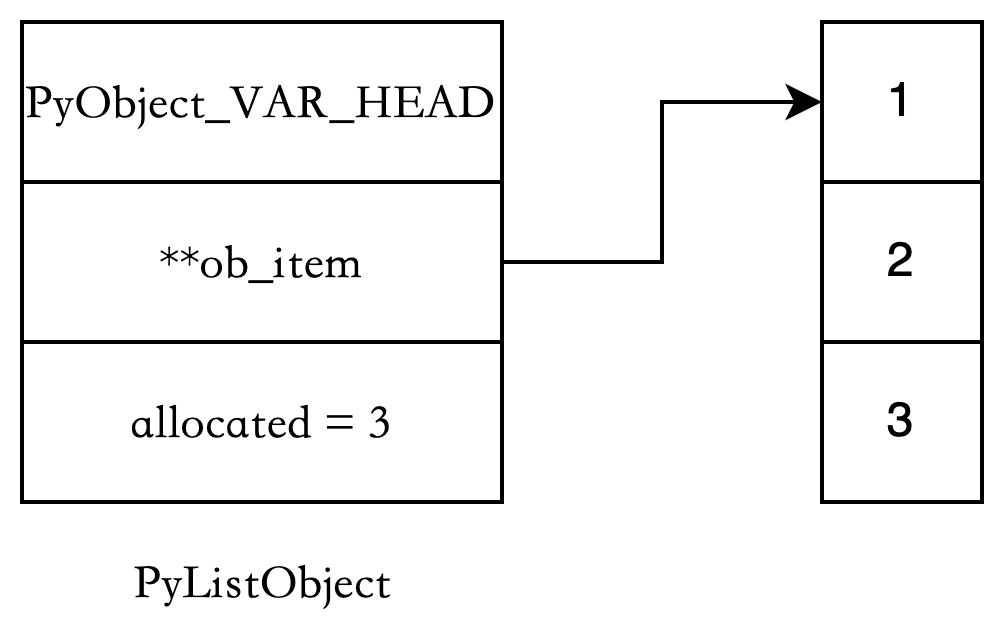
\includegraphics[width=0.5\textwidth]{pictures/ch7_01.png}
  \caption{含有三个元素的 PyListObject \label{fig:scatter}}
\end{figure}

\section{创建 List}

创建 List 是在写 Python 代码时的一个使用频率非常高的操作。一般有两种写法。

\begin{lstlisting}[language=Python, numbers=left, numbersep=1em, numberstyle=\footnotesize , breaklines=true]
a = list()
b = []
\end{lstlisting}

这两种写法最后都会调用 PyList\_New 函数来创建一个  PyListObject 对象。所以看一下 PyList\_New 函数究竟是如何创建一个 List 的。

\begin{lstlisting}[language=C, numbers=left, numbersep=1em, numberstyle=\footnotesize , breaklines=true]
PyObject *
PyList_New(Py_ssize_t size)
{
    // 处理参数错误
    if (size < 0) {
        PyErr_BadInternalCall();
        return NULL;
    }

    struct _Py_list_state *state = get_list_state();
    PyListObject *op;
    // 如果空闲链表中有元素,直接取空闲链表中的元素
    if (state->numfree) {
        state->numfree--;
        op = state->free_list[state->numfree];
        _Py_NewReference((PyObject *)op);
    }
    else {
        // 对 PyList_Type 类型进行 GC,从被释放的元素中获取一个 PyListObject
        op = PyObject_GC_New(PyListObject, &PyList_Type);
        if (op == NULL) {
            return NULL;
        }
    }
    if (size <= 0) {
        op->ob_item = NULL;
    }
    else {
       // 如果参数 size > 0,则申请需要的内存,ob_item 指向申请的内存
        op->ob_item = (PyObject **) PyMem_Calloc(size, sizeof(PyObject *));
        if (op->ob_item == NULL) {
            Py_DECREF(op);
            return PyErr_NoMemory();
        }
    }
    // 设置 ob_size = size
    Py_SET_SIZE(op, size);
    // 设置数组数量
    op->allocated = size;
    _PyObject_GC_TRACK(op);
    return (PyObject *) op;
}
\end{lstlisting}

可以看到,创建一个 List 的过程也是很简洁的,里面提到的 GC 在后面章节会进行详细描述,这里暂且跳过不表。

\section{List 的类型类}

List 的类型类是 PyList\_Type,下面是它的定义。

\begin{lstlisting}[language=C, numbers=left, numbersep=1em, numberstyle=\footnotesize , breaklines=true]
PyTypeObject PyList_Type = {
    PyVarObject_HEAD_INIT(&PyType_Type, 0)
    "list",
    sizeof(PyListObject),
    0,
    (destructor)list_dealloc,                   /* tp_dealloc */
    0,                                          /* tp_vectorcall_offset */
    0,                                          /* tp_getattr */
    0,                                          /* tp_setattr */
    0,                                          /* tp_as_async */
    (reprfunc)list_repr,                        /* tp_repr */
    0,                                          /* tp_as_number */
    &list_as_sequence,                          /* tp_as_sequence */
    &list_as_mapping,                           /* tp_as_mapping */
    PyObject_HashNotImplemented,                /* tp_hash */
    0,                                          /* tp_call */
    0,                                          /* tp_str */
    PyObject_GenericGetAttr,                    /* tp_getattro */
    0,                                          /* tp_setattro */
    0,                                          /* tp_as_buffer */
    Py_TPFLAGS_DEFAULT | Py_TPFLAGS_HAVE_GC |
        Py_TPFLAGS_BASETYPE | Py_TPFLAGS_LIST_SUBCLASS |
        _Py_TPFLAGS_MATCH_SELF | Py_TPFLAGS_SEQUENCE,  /* tp_flags */
    list___init____doc__,                       /* tp_doc */
    (traverseproc)list_traverse,                /* tp_traverse */
    (inquiry)_list_clear,                       /* tp_clear */
    list_richcompare,                           /* tp_richcompare */
    0,                                          /* tp_weaklistoffset */
    list_iter,                                  /* tp_iter */
    0,                                          /* tp_iternext */
    list_methods,                               /* tp_methods */
    0,                                          /* tp_members */
    0,                                          /* tp_getset */
    0,                                          /* tp_base */
    0,                                          /* tp_dict */
    0,                                          /* tp_descr_get */
    0,                                          /* tp_descr_set */
    0,                                          /* tp_dictoffset */
    (initproc)list___init__,                    /* tp_init */
    PyType_GenericAlloc,                        /* tp_alloc */
    PyType_GenericNew,                          /* tp_new */
    PyObject_GC_Del,                            /* tp_free */
    .tp_vectorcall = list_vectorcall,
};
\end{lstlisting}

看起来内容很多,但其实我们并不需要了解这么多。在本章节中,需要关注的元素就如下几个。

\begin{lstlisting}[language=C, numbers=left, numbersep=1em, numberstyle=\footnotesize , breaklines=true]
PyTypeObject PyList_Type = {
    PyVarObject_HEAD_INIT(&PyType_Type, 0)
    "list",
    sizeof(PyListObject),
    0,                                          /* tp_as_number */
    &list_as_sequence,                          /* tp_as_sequence */
    &list_as_mapping,                           /* tp_as_mapping */
    PyObject_HashNotImplemented,                /* tp_hash */
};
\end{lstlisting}

其中 list\_as\_sequence 是 List 作为序列时调用的方法集合,list\_as\_mapping 是 List 作为映射时调用的方法集合,
PyObject\_HashNotImplemented 也值得一看,因为 List 是一个可变的类型,所以在 Python 中,List 是不可以作为
字典的 key 的,如果尝试将 List 作为 key,会爆一个类型错误。

\begin{lstlisting}[language=Python, numbers=left, numbersep=1em, numberstyle=\footnotesize , breaklines=true]
>>> d = {}
>>> d[[233]] = "bilibili"
Traceback (most recent call last):
  File "<stdin>", line 1, in <module>
TypeError: unhashable type: 'list'
\end{lstlisting}

而这个错误恰恰就是 PyObject\_HashNotImplemented 抛出的。

\begin{lstlisting}[language=C, numbers=left, numbersep=1em, numberstyle=\footnotesize , breaklines=true]
Py_hash_t
PyObject_HashNotImplemented(PyObject *v)
{
    PyErr_Format(PyExc_TypeError, "unhashable type: '%.200s'",
                 Py_TYPE(v)->tp_name);
    return -1;
}
\end{lstlisting}

\section{List 部分方法的实现}

要知道 List 中的方法是如何实现的,就需要去了解一下上一节中提到的 list\_as\_sequence 和 list\_as\_mapping 成员。
针对 List 调用的大部分函数都是实现在这两个成员中。List 在 Python 中是同时作为一个序列和一个映射的,所以可以看一下
 List 实现了这两种类型中哪些函数。具体这两个类型每个成员分别表示什么操作可以通过章末列出的资料去了解,这里不一一阐述。

\begin{lstlisting}[language=C, numbers=left, numbersep=1em, numberstyle=\footnotesize , breaklines=true]
static PySequenceMethods list_as_sequence = {
    (lenfunc)list_length,                       /* sq_length */
    (binaryfunc)list_concat,                    /* sq_concat */
    (ssizeargfunc)list_repeat,                  /* sq_repeat */
    (ssizeargfunc)list_item,                    /* sq_item */
    0,                                          /* sq_slice */
    (ssizeobjargproc)list_ass_item,             /* sq_ass_item */
    0,                                          /* sq_ass_slice */
    (objobjproc)list_contains,                  /* sq_contains */
    (binaryfunc)list_inplace_concat,            /* sq_inplace_concat */
    (ssizeargfunc)list_inplace_repeat,          /* sq_inplace_repeat */
};

static PyMappingMethods list_as_mapping = {
    (lenfunc)list_length,
    (binaryfunc)list_subscript,
    (objobjargproc)list_ass_subscript
};
\end{lstlisting}

\subsection{List 的长度}

获取 List 的长度的常用方法是 len() 函数,底层调用的是 list\_length 函数,直接返回 ob\_size 成员。
\begin{lstlisting}[language=C, numbers=left, numbersep=1em, numberstyle=\footnotesize , breaklines=true]
static Py_ssize_t
list_length(PyListObject *a)
{
    return Py_SIZE(a);
}
\end{lstlisting}

\subsection{获取 List 某个位置的元素}

获取 List 某个位置的元素的函数用法一般是下面这样子。

\begin{lstlisting}[language=Python, numbers=left, numbersep=1em, numberstyle=\footnotesize , breaklines=true]
a = [3, 2, 1]
a[1]  # 2
a[0:2] # [0, 1]
\end{lstlisting}

其中 a[1] 就是获取 List a 的 第2 个位置的元素(元素位置从 0 开始计数)。底层函数是 list\_item。

\begin{lstlisting}[language=C, numbers=left, numbersep=1em, numberstyle=\footnotesize , breaklines=true]
static PyObject *
list_item(PyListObject *a, Py_ssize_t i)
{
    if (!valid_index(i, Py_SIZE(a))) {
        if (indexerr == NULL) {
            indexerr = PyUnicode_FromString(
                "list index out of range");
            if (indexerr == NULL)
                return NULL;
        }
        PyErr_SetObject(PyExc_IndexError, indexerr);
        return NULL;
    }
    Py_INCREF(a->ob_item[i]);
    return a->ob_item[i];
}
\end{lstlisting}

a[0:2] 是获取 List 中某个区间的元素,底层调用的是 List 作为映射类型的一个方法 list\_subscript。
\begin{lstlisting}[language=C, numbers=left, numbersep=1em, numberstyle=\footnotesize , breaklines=true]
static PyObject *
list_subscript(PyListObject* self, PyObject* item)
{
    if (_PyIndex_Check(item)) {
        Py_ssize_t i;
        i = PyNumber_AsSsize_t(item, PyExc_IndexError);
        if (i == -1 && PyErr_Occurred())
            return NULL;
        if (i < 0)
            i += PyList_GET_SIZE(self);
        return list_item(self, i);
    }
    // 如果是取数组的范围,那么 item 的类型是 slice
    else if (PySlice_Check(item)) {
        Py_ssize_t start, stop, step, slicelength, i;
        size_t cur;
        PyObject* result;
        PyObject* it;
        PyObject **src, **dest;
        // 取出开始 结尾和步长
        if (PySlice_Unpack(item, &start, &stop, &step) < 0) {
            return NULL;
        }
        // 求需要返回的元素个数,可以简单理解为 (stop - start - 1) / step + 1
        slicelength = PySlice_AdjustIndices(Py_SIZE(self), &start, &stop,
                                            step);
        // start = stop, step = 1 的情况
        if (slicelength <= 0) {
            return PyList_New(0);
        }
        // 如果 step = 1,直接返回 List[start, stop)
        else if (step == 1) {
            return list_slice(self, start, stop);
        }
        else {
            // 如果 step > 1,那么闲创建一个 List, 再将对应位置的元素插入到创建的 List
            result = list_new_prealloc(slicelength);
            if (!result) return NULL;

            src = self->ob_item;
            dest = ((PyListObject *)result)->ob_item;
            for (cur = start, i = 0; i < slicelength;
                 cur += (size_t)step, i++) {
                it = src[cur];
                Py_INCREF(it);
                dest[i] = it;
            }
            Py_SET_SIZE(result, slicelength);
            return result;
        }
    }
    else {
        PyErr_Format(PyExc_TypeError,
                     "list indices must be integers or slices, not %.200s",
                     Py_TYPE(item)->tp_name);
        return NULL;
    }
}
\end{lstlisting}

\subsection{设置 List 的元素}

设置 List 的元素和获取 List 的元素一样,也分为两种情况,分别是一次设置一个位置上的元素
和一次设置多个位置上的元素。和获取元素不同的是,这两种情况的入口函数只有一个,都是
映射类型的方法 list\_ass\_subscript。

\begin{lstlisting}[language=Python, numbers=left, numbersep=1em, numberstyle=\footnotesize , breaklines=true]
a = [3, 2, 1]
a[1] = 100
a[0:2] = []
\end{lstlisting}

\begin{lstlisting}[language=C, numbers=left, numbersep=1em, numberstyle=\footnotesize , breaklines=true]
static int
list_ass_subscript(PyListObject* self, PyObject* item, PyObject* value)
{
    // 如果是 a[1] = 100 这种语法,则进入下面这个分支
    if (_PyIndex_Check(item)) {
        Py_ssize_t i = PyNumber_AsSsize_t(item, PyExc_IndexError);
        if (i == -1 && PyErr_Occurred())
            return -1;
        if (i < 0)
            i += PyList_GET_SIZE(self);
        // 调用序列类型的方法设置位置 i 的值为 value
        return list_ass_item(self, i, value);
    }
    // 如果是 a[0:2] = [] 这种语法,则进入下面这个分支
    else if (PySlice_Check(item)) {
        Py_ssize_t start, stop, step, slicelength;

        if (PySlice_Unpack(item, &start, &stop, &step) < 0) {
            return -1;
        }
        slicelength = PySlice_AdjustIndices(Py_SIZE(self), &start, &stop,
                                            step);
        // 如果是 a[0:2] = [], 这种形式,把 a[0:2] 替换为 []
        if (step == 1)
            return list_ass_slice(self, start, stop, value);
        // 处理 s[5:2] = [..] 这种开始位置大于结束位置的情况
        // 将结束位置改为开始位置,相当于在开始位置之后插入
        if ((step < 0 && start < stop) ||
            (step > 0 && start > stop))
            stop = start;
        // 这种情况下直接删除选中的 List 区域,但是不知道怎么构造这个例子
        if (value == NULL) {
            /* delete slice */
            PyObject **garbage;
            size_t cur;
            Py_ssize_t i;
            int res;

            if (slicelength <= 0)
                return 0;

            if (step < 0) {
                stop = start + 1;
                start = stop + step*(slicelength - 1) - 1;
                step = -step;
            }

            garbage = (PyObject**)
                PyMem_Malloc(slicelength*sizeof(PyObject*));
            if (!garbage) {
                PyErr_NoMemory();
                return -1;
            }
            for (cur = start, i = 0;
                 cur < (size_t)stop;
                 cur += step, i++) {
                Py_ssize_t lim = step - 1;

                garbage[i] = PyList_GET_ITEM(self, cur);

                if (cur + step >= (size_t)Py_SIZE(self)) {
                    lim = Py_SIZE(self) - cur - 1;
                }

                memmove(self->ob_item + cur - i,
                    self->ob_item + cur + 1,
                    lim * sizeof(PyObject *));
            }
            cur = start + (size_t)slicelength * step;
            if (cur < (size_t)Py_SIZE(self)) {
                memmove(self->ob_item + cur - slicelength,
                    self->ob_item + cur,
                    (Py_SIZE(self) - cur) *
                     sizeof(PyObject *));
            }

            Py_SET_SIZE(self, Py_SIZE(self) - slicelength);
            res = list_resize(self, Py_SIZE(self));

            for (i = 0; i < slicelength; i++) {
                Py_DECREF(garbage[i]);
            }
            PyMem_Free(garbage);

            return res;
        }
        else {
            // 处理 a[0:20:2] = [..] 这种情况
            PyObject *ins, *seq;
            PyObject **garbage, **seqitems, **selfitems;
            Py_ssize_t i;
            size_t cur;

            /* protect against a[::-1] = a */
            if (self == (PyListObject*)value) {
                seq = list_slice((PyListObject*)value, 0,
                                   PyList_GET_SIZE(value));
            }
            else {
                seq = PySequence_Fast(value,
                                      "must assign iterable "
                                      "to extended slice");
            }
            if (!seq)
                return -1;

            if (PySequence_Fast_GET_SIZE(seq) != slicelength) {
                PyErr_Format(PyExc_ValueError,
                    "attempt to assign sequence of "
                    "size %zd to extended slice of "
                    "size %zd",
                         PySequence_Fast_GET_SIZE(seq),
                         slicelength);
                Py_DECREF(seq);
                return -1;
            }

            if (!slicelength) {
                Py_DECREF(seq);
                return 0;
            }

            garbage = (PyObject**)
                PyMem_Malloc(slicelength*sizeof(PyObject*));
            if (!garbage) {
                Py_DECREF(seq);
                PyErr_NoMemory();
                return -1;
            }

            selfitems = self->ob_item;
            seqitems = PySequence_Fast_ITEMS(seq);
            for (cur = start, i = 0; i < slicelength;
                 cur += (size_t)step, i++) {
                garbage[i] = selfitems[cur];
                ins = seqitems[i];
                Py_INCREF(ins);
                selfitems[cur] = ins;
            }

            for (i = 0; i < slicelength; i++) {
                Py_DECREF(garbage[i]);
            }

            PyMem_Free(garbage);
            Py_DECREF(seq);

            return 0;
        }
    }
    else {
        PyErr_Format(PyExc_TypeError,
                     "list indices must be integers or slices, not %.200s",
                     Py_TYPE(item)->tp_name);
        return -1;
    }
}
\end{lstlisting}

设置 List 元素的函数还是比较复杂的,不过以不同的参数分为了几类主要的情况,都在上面进行了介绍。

\section{List 添加元素}

List 可以使用 append 和 extend 方法来添加元素,接下来就分析下这两个方法的细节。

\begin{lstlisting}[language=Python, numbers=left, numbersep=1em, numberstyle=\footnotesize , breaklines=true]
>>> a = []
>>> a.append([1,2,3])
>>> a
[[1, 2, 3]]
>>> a.extend([4,5,6])
>>> a
[[1, 2, 3], 4, 5, 6]
\end{lstlisting}

append 方法会在原来的 List 对象后面添加一个新元素,不过每次只能添加一个。
extend 方法则是将新的元素“解包”之后再添加到原来的 List 的最后面。

append 方法的实现相对来说比较简单,毕竟每次只需要考虑添加一个元素。所以代码
也比较简洁,主要分为两步。第一步检查是否需要扩容,如果需要的话,进行扩容。
第二步是将 append 的参数(一个 PyObject)添加到原本的 List 数组的末尾。
\begin{lstlisting}[language=C, numbers=left, numbersep=1em, numberstyle=\footnotesize , breaklines=true]
static PyObject *
list_append(PyListObject *self, PyObject *object)
{
    if (app1(self, object) == 0)
        Py_RETURN_NONE;
    return NULL;
}

static int
app1(PyListObject *self, PyObject *v)
{
    Py_ssize_t n = PyList_GET_SIZE(self);

    assert (v != NULL);
    assert((size_t)n + 1 < PY_SSIZE_T_MAX);
    // 数组扩容,不一定会发生在次分配
    if (list_resize(self, n+1) < 0)
        return -1;

    Py_INCREF(v);
    // 将新的 PyObject 添加到数组的最后面
    PyList_SET_ITEM(self, n, v);
    return 0;
}
\end{lstlisting}

extend 方法相比于 append 方法要复杂一些。主要是因为 extend 方法的参数可能性比较多,list、tuple,
和一些可迭代的对象类似于 set 等都可以作为 extend 方法的参数。大体情况分两种,第一种是 如果参数
是 list、tuple 对象或者 list 自身,那么先扩容,再将参数的所有成员添加到本 list 对象的数组中。第二种
情况是如果参数是一个可迭代对象,那么先获取可迭代对象的数量,对本 list 进行扩容,接着遍历一次可
迭代对象,将所有成员添加到本 list 的数组中。

\begin{lstlisting}[language=C, numbers=left, numbersep=1em, numberstyle=\footnotesize , breaklines=true]
static PyObject *
list_extend(PyListObject *self, PyObject *iterable)
{
    PyObject *it;      /* iter(v) */
    Py_ssize_t m;                  /* size of self */
    Py_ssize_t n;                  /* guess for size of iterable */
    Py_ssize_t mn;                 /* m + n */
    Py_ssize_t i;
    PyObject *(*iternext)(PyObject *);
    // 如果 iterable 参数是 List, Tuple 类型,或者是 List 自身(那么当然也是一个 List 了,所以为什么还
    // 要检查self == iterable),就进入下面这个分支
    if (PyList_CheckExact(iterable) || PyTuple_CheckExact(iterable) ||
                (PyObject *)self == iterable) {
        PyObject **src, **dest;
        // 如果 iterable 是一个 List 或者 Tuple 的话,iterable 还是自身
        // 如果是一个可迭代对象的话,
        iterable = PySequence_Fast(iterable, "argument must be iterable");
        if (!iterable)
            return NULL;
        n = PySequence_Fast_GET_SIZE(iterable);
        if (n == 0) {
            /* short circuit when iterable is empty */
            Py_DECREF(iterable);
            Py_RETURN_NONE;
        }
        m = Py_SIZE(self);
        assert(m < PY_SSIZE_T_MAX - n);
        // 数组扩容
        if (list_resize(self, m + n) < 0) {
            Py_DECREF(iterable);
            return NULL;
        }
        src = PySequence_Fast_ITEMS(iterable);
        dest = self->ob_item + m;
        // 将 iterable 内的元素全部添加到 List 的数组之后
        for (i = 0; i < n; i++) {
            PyObject *o = src[i];
            Py_INCREF(o);
            dest[i] = o;
        }
        Py_DECREF(iterable);
        Py_RETURN_NONE;
    }
    // iterable 是一个类似 set 的可迭代对象,则进入下面的分支
    it = PyObject_GetIter(iterable);
    if (it == NULL)
        return NULL;
    iternext = *Py_TYPE(it)->tp_iternext;

    // 获取 iterable 中元素数量
    n = PyObject_LengthHint(iterable, 8);
    if (n < 0) {
        Py_DECREF(it);
        return NULL;
    }
    m = Py_SIZE(self);
    if (m > PY_SSIZE_T_MAX - n) {
         // 如果进入了这个分支,那么要不然是 n 的值错误了,不用管
         // 要不然最后肯定会在下面的循环中导致系统内存消耗完,救不了
    }
    else {
        mn = m + n;
        // 扩容
        if (list_resize(self, mn) < 0)
            goto error;
        Py_SET_SIZE(self, m);
    }

    // 将 iterable 内的元素全部添加到 List 的数组之后
    for (;;) {
        PyObject *item = iternext(it);
        if (item == NULL) {
            if (PyErr_Occurred()) {
                if (PyErr_ExceptionMatches(PyExc_StopIteration))
                    PyErr_Clear();
                else
                    goto error;
            }
            break;
        }
        if (Py_SIZE(self) < self->allocated) {
            /* steals ref */
            PyList_SET_ITEM(self, Py_SIZE(self), item);
            Py_SET_SIZE(self, Py_SIZE(self) + 1);
        }
        else {
            int status = app1(self, item);
            Py_DECREF(item);  /* append creates a new ref */
            if (status < 0)
                goto error;
        }
    }

    // 一个小优化,如果上面扩容阔的太大了,这里再进行缩容,不过感觉是多此一举
    if (Py_SIZE(self) < self->allocated) {
        if (list_resize(self, Py_SIZE(self)) < 0)
            goto error;
    }

    Py_DECREF(it);
    Py_RETURN_NONE;

  error:
    Py_DECREF(it);
    return NULL;
}
\end{lstlisting}

\section{List 排序}



\section{参考}

\begin{itemize}
\item \href{https://docs.python.org/3/c-api/typeobj.html}{Type Objects}
\end{itemize}



 % Python List 对象
%%%%%%%%%%%%%%%%%%%%%%%%%%%%%%%%%%%%%%%%%%%%%%%%%%%%%%%%%
%%%  Dict 对象
%%%%%%%%%%%%%%%%%%%%%%%%%%%%%%%%%%%%%%%%%%%%%%%%%%%%%%%%%

\chapter{Python Dict 对象} % Python Dict 对象
%%%%%%%%%%%%%%%%%%%%%%%%%%%%%%%%%%%%%%%%%%%%%%%%%%%%
%%% Python 字节码
%%%%%%%%%%%%%%%%%%%%%%%%%%%%%%%%%%%%%%%%%%%%%%%%%%%%

\chapter{Python 字节码}

\section{line number table}

Python 需要一个对照表结构来表明字节码和源代码的对照关系。最简单来说,要实现这样子一张对照表,
需要对每行 Python 源代码需要三个字段。字节码开始位置,字节码结束位置,该段字节码对应的源代码
行,需要源代码行的原因是源代码并不是每一行都有内容,而是可能会存在空行。

考虑如下最简单的对照表

\begin{lstlisting}[language=C, numbers=left, numbersep=1em, numberstyle=\footnotesize , breaklines=true]
     Start    End     Line
      0       6       1
      6       50      2
      50      350     7
      350     360     No line number
      360     376     8
      376     380     208
\end{lstlisting}

如果 Start, End, Line 每一个字段都用 4 字节来表示的话,那么每一行就需要 12 字节,这个内存消耗显然
太大了,所以需要压缩存储对照表使用的内存空间。可以发现,上表中,每一行的 End 等于下一行的 Start,
每一行的 Line 也可以改为相对上一行 Line 的偏移(第一行的 Line 一定是相对于 0 来计算的),那么每一行
就可以改为两列 (End - Start, Line 相对上一行的偏移),所以可以得出下面这个偏移表。

\begin{lstlisting}[language=C, numbers=left, numbersep=1em, numberstyle=\footnotesize , breaklines=true]
   End-Start  Line-delta
      6         +1
      44        +1
      300       +5
      10        No line number
      16        +1
      4         +200
\end{lstlisting}

这个更改减少了一列,节约了 $\frac{1}{3}$ 的空间。但是还可以继续优化,在实际的代码中,我们发现,End - Start
 和 Line 相对上一行的偏移大部分情况下都是一个小整数,所以,End - Start 和 Line-delta 都应该可以优化为用一个字节
 表示。End-Start 可以优化为一个 [0, 254] 的整数,Line-delta 可以优化为 [-128, 127] 的整数,Line-delta 的 -128 用来表示
 这一列没有行号,0 表示这一列没有字节码(实质上是用来分解上一列的 End-Start 的,因为每一列的 End-Start 允许的
 最大值为 254,超过了这个值,就需要分解为多行)。在这个限制条件下,可以得出第三种对照表,这个对照表就是内存
 中最后实际存储的对照表。在这个条件下,对照表每一列只需要两字节的存储空间,在最优的情况下,相比于原版每一列
 12 字节,节约了 $\frac{5}{6}$ 的空间。
 
\begin{lstlisting}[language=C, numbers=left, numbersep=1em, numberstyle=\footnotesize , breaklines=true]
    Start delta   Line delta
    6               +1
    44              +1
    254             +5
    46              0     // 上一列的 START delta 为 300,超过了 254 的上限,所以需要分解为 254 + 46 两列
    10              -128 (No line number, treated as a delta of zero)
    16              +1
    0               +127 (line 135, but the range is empty as no bytecodes are at line 135)
    4               +73 // 上一列的 Line delta 为 200,超过了 127 的上限,所以需要分解为 127 + 73 两列
\end{lstlisting}














 % Python 字节码

%
%
%\chapter{Python dict 对象}
%
%\section{参考资料}
%
%本节列一下参考资料。
%
%
%
%\chapter{pyc 文件分析}
%
%本节介绍一下 Python pyc 文件的相关信息。
%
%\section{参考资料}
%
%本节列一下参考资料。
%
%
%\chapter{Python 虚拟机框架}
%
%本章介绍一下 Python 虚拟机的基本框架。
%
%\section{参考资料}
%
%本节列一下参考资料。
%
%
%\chapter{Python 虚拟机中的一般表达式}
%
%本章介绍一下 Python 虚拟机中的一般表达式的处理。
%
%\section{参考资料}
%
%本节列一下参考资料。
%
%
%\chapter{Python虚拟机中的控制流}
%
%本章介绍一下 Python 虚拟机中的控制流。
%
%\section{参考资料}
%
%本节列一下参考资料。
%
%
%\chapter{Python 虚拟机中的函数}
%
%本章介绍一下 Python 虚拟机中函数的实现。
%
%\section{参考资料}
%
%本节列一下参考资料。
%
%
%\chapter{Python 虚拟机中的类}
%
%本章介绍一下 Python 虚拟机中类的实现。
%
%\section{meta class}
%
%本节介绍一下 Python 虚拟机中元类的实现。
%
%\section{参考资料}
%
%本节列一下参考资料。
%
%
%\chapter{Python 运行环境初始化过程}
%
%本章介绍一下 Python 运行环境初始化的过程。
%
%\section{参考资料}
%
%本节列一下参考资料。
%
%
%\chapter{Python 模块的加载机制}
%
%本章介绍一下 Python 模块的加载机制。
%
%\section{参考资料}
%
%本节列一下参考资料。
%
%
%
%\chapter{Python 多线程机制}
%
%本章介绍一下 Python 多线程机制。
%
%\section{参考资料}
%
%本节列一下参考资料。
%
%
%
%\chapter{Python 内存管理机制}
%
%本章介绍一下 Python 内存管理机制。
%
%\section{参考资料}
%
%本节列一下参考资料。
%
%
%
%\chapter{Python C 拓展}
%
%本章介绍一下 Python 的 C 拓展的解析机制。
%
%\section{参考资料}
%
%本节列一下参考资料。
%
%
%
%\chapter{Python trackback 机制}
%
%本章介绍一下 Python 的 trackback 机制。
%
%\section{参考资料}
%
%本节列一下参考资料。
%
%
%
%\chapter{Python 热更新机制}
%
%本章介绍一下 Python 的热更新机制。
%
%\section{参考资料}
%
%本节列一下参考资料。
%
%
%



\end{document}
